\pdfbookmark{Общая характеристика работы}{characteristic}             % Закладка pdf
\section*{Общая характеристика работы}

\newcommand{\actuality}{\pdfbookmark[1]{Актуальность}{actuality}\underline{\textbf{\actualityTXT}}}
\newcommand{\progress}{\pdfbookmark[1]{Разработанность темы}{progress}\underline{\textbf{\progressTXT}}}

\newcommand{\objectresearch}{\pdfbookmark[1]{Объект исследования}{progress}\underline{\textbf{\objectresearchTXT}}}

\newcommand{\subjectresearch}{\pdfbookmark[1]{Предмет исследования}{progress}\underline{\textbf{\subjectresearchTXT}}}

\newcommand{\aim}{\pdfbookmark[1]{Цели}{aim}\underline{{\textbf\aimTXT}}}
\newcommand{\tasks}{\pdfbookmark[1]{Задачи}{tasks}\underline{\textbf{\tasksTXT}}}
\newcommand{\aimtasks}{\pdfbookmark[1]{Цели и задачи}{aimtasks}\aimtasksTXT}
\newcommand{\novelty}{\pdfbookmark[1]{Научная новизна}{novelty}\underline{\textbf{\noveltyTXT}}}

\newcommand{\fieldresearch}{\pdfbookmark[1]{Область исследования}{fieldresearch}\underline{\textbf{\fieldresearchTXT}}}

\newcommand{\influence}{\pdfbookmark[1]{Практическая значимость}{influence}\underline{\textbf{\influenceTXT}}}
\newcommand{\elaboration}{\pdfbookmark[1]{Степень разработанности темы}{elaboration}\underline{\textbf{\elaborationTXT}}}
\newcommand{\methods}{\pdfbookmark[1]{Методы исследования}{methods}\underline{\textbf{\methodsTXT}}}
\newcommand{\defpositions}{\pdfbookmark[1]{Положения, выносимые на защиту}{defpositions}\underline{\textbf{\defpositionsTXT}}}
\newcommand{\reliability}{\pdfbookmark[1]{Достоверность}{reliability}\underline{\textbf{\reliabilityTXT}}}
\newcommand{\probation}{\pdfbookmark[1]{Апробация}{probation}\underline{\textbf{\probationTXT}}}
\newcommand{\contribution}{\pdfbookmark[1]{Личный вклад}{contribution}\underline{\textbf{\contributionTXT}}}
\newcommand{\publications}{\pdfbookmark[1]{Публикации}{publications}\underline{\textbf{\publicationsTXT}}}

{\actuality} 

% В настоящее время заметна тенденция цифровой трансформации, что подразумевает под собой бурное развитие информационных технологий во всех сферах деятельности человека. Основными перспективными направлениями цифровизации, на которые сделан акцент в диссертационной работе, являются цифровая трансформация транспортного комплекса и глобальная цифровизация нефтегазового сектора страны. Этот подход подразумевает не только оснащение современным технологичным оборудованием, но и глобальное изменение в подходах управления, сбора информации и средств коммуникаций. Уже сейчас основными современными информационными технологиями, встречающимися на пути трансформации являются: большие данные (Big Data), предиктивные модели на искусственных нейронных сетях (Artificial Neural Network), системы распределенного реестра (Blockchain), промышленный интернет вещей (Industrial Internet of Things, IIoT), технологии виртуальной и дополненной реальности (Virtual Reality, VR), мониторинг распределенных объектов с помощью беспилотных летательных аппаратов БПЛА (Unmanned Aerial Vehicle, UAV). В совокупности данные технологии создают необходимость в эффективной передаче больших объемов высокоскоростного трафика. Одним из путей решенияй проблемы является интенсивное развитие и внедрение беспроводных технологий.

% \fixme{В настоящее время заметна тенденция бурного развития информационных технологий во всех сферах деятельности человека. На сегодня 

% оказывает весомое влияние на нефтегазовый сектор страны. Современные компании, представляющие собой сложные многоуровневые производственные системы, для своего устойчивого развития требуют постоянного развития и совершенствования передовых технологий.  Сегодня наблюдается  бурное развитие процесса «цифровизации» нефтегазовой отрасли. Крупные международные нефтегазовые компании имеют подразделения, задачами которых является разработка и реализация принципов интеллектуального месторождения \cite{Tcharo2018} на промысле, организация безопасности на технологических объектах, развитие концепции  перехода к малолюдным системам управления добычей, транспортировкой и переработкой сырья. Уже сейчас основными современными информационными технологиями, встречающиеся в отрасли являются: большие данные (Big Data), предикстивные модели на искусственных нейронных сетях (Artificial Neural Network), системы распределенного реестра (Blockchain), промышленный интернет вещей (Industrial internet of things, IIoT), технологии виртуальной и дополненной реальности (Virtual Reality, VR), мониторинг распределенных объектов с помощью беспилотных летательных аппаратов БПЛА (Unmanned Aerial Vehicle, UAV). }
 
 
% \fixme{В совокупности данные технологии создают необходимость эффективной передачи больших объемов высокоскоростного трафика. Информационные  системы современных  сегодня содержат колоссальный объем информации высокоскоростного мультимедийного трафика. Одним из путей решения является внедрение беспроводных технологий.}

Создание современной инфраструктуры передачи данных вдоль транспортных магистралей является одной из важнейших проблем при создании нового и функционировании существующего транспортного комплекса  \cite{Vishnevsky2016_Review_of_methodology}. Одним из путей решения проблемы является интенсивное развитие и внедрение беспроводных технологий. Активное использование беспроводных сетей основывается на ряде их преимуществ по сравнению с кабельными сетями:
\begin{itemize}
    \item организация связи в труднодоступных регионах;
    \item быстрый ввод в эксплуатацию по системе подключение типа <<Подключил и Работай>> (Plug-\&-Play);
    \item сокращение капитальных затрат на создание сети; 
    \item уменьшение затрат на эксплуатацию;
    \item высокая гибкость, мобильность, масштабируемость;
    \item упрощенные требования к обслуживанию оборудования.
\end{itemize}

В рамках этого процесса возникает актуальная научно-техническая проблема повышения качества топологического проектирования беспроводной сети связи, осуществляющей мониторинг, сбор и передачу информации в центр управления с множества объектов на заданной территории.   

% В совокупности со всеми вышеизложенными перспективными направлениями беспроводные технологии являются неотъемлемой частью «цифровизации» месторождения. Отсюда возникает научно - техническая проблема организации распределенной беспроводной сети связи, соответствующая реальным требованием современного производства.

% Большой объем передачи информации  привел к еще одной из наиболее интересных тенденций цифрового развития – внедрения беспроводных технологий. Современные месторождения сегодня, помимо данных первичного сбора и обработки информации технологических параметров основных производственных объектов содержат также колоссальный объем  информации мультимедийного трафика. Сюда входят данные БПЛА по обнаружению утечек и  разрушения трубопроводов; камер видеонаблюдений; а также большой поток данных цифровых двойников, аналитики и т.д. В совокупности со всеми вышеизложенными перспективными направлениями беспроводные технологии являются неотъемлемой частью «цифровизации» месторождения.



% Процесс проектирования современной  беспроводной сети связи состоит из последовательного решения взаимосвязанных задач:

% \begin{enumerate}
%     \item обследование местности;
%     \item выбор типов технических средств и протоколов;
%     \item выбор топологической структуры сети;
%     \item анализ и оценка будущей беспроводной сети с помощью математического моделирования.
% \end{enumerate}

Диссертация посвящена актуальной проблеме синтеза топологической структуры беспроводной широкополосной сети. Задача выбора топологической структуры при проектировании является одной из важнейших задач, ошибки при которой могут привести к большим капитальным затратам и ухудшению качества обслуживания (Quality Of Service, QoS). С математической точки зрения задача синтеза топологии является сложной задачей, время счета для которой растет экспоненциально с ростом размерности. Таким образом, высокий теоретический и практический интерес к разработке новых моделей и методов оптимизации топологической структуры беспроводной широкополосной сети определяет актуальность и новизну диссертационной работы.


% Задача синтеза топологии при комплексном проектировании БШС является основной проблемой исследования в данной работе.

% В.М. Вишневский, Ю. В. Гайдамака, А.Е. Кучерявый, А.А. Ларионов, В.М. Малыш,  О.Ю. Першин, К. Е. Самуйлов, Р.Л. Смелянский и другие.

% Создание и постоянное развитие современной инфраструктуры передачи данных является одной из основных задач цифровизации. Бурное развитие беспроводных сетей во всех областях деятельности человека: интеллектуальные транспортные системы вдоль автомобильных дорог, мониторинг нефтегазовых объектов, организация современного высокоскоростного покрытия в общественных зонах обосновывают целесообразность их использования. 

% и, в частности, решающие задачу синтеза топологии В. М. Вишневский, А. А. Ларионов, В.М. Малыш, О. Ю. Першин.

{\progress} В настоящее время в России и за рубежом исследованию беспроводных сетей связи посвящен ряд работ, где рассматриваются сети для мониторинга гражданских  и промышленных объектов. Примерами таких объектов является жилые районы города, протяженные автомагистрали, линии метрополитена и железные дороги, магистральные трубопроводы и др. При исследовании проблемы синтеза топологии сети автор опирался на труды отечественных ученых, занимающихся исследованиями в области телекоммуникационных сетей: В.М. Вишневский, Ю. В. Гайдамака, Р.В. Киричек, А. Е. Кучерявый, Е. А. Кучерявый, А. А. Ларионов, В. М. Малыш,  О. Ю. Першин, К. Е. Самуйлов, Р. Л. Смелянский. Наряду с отечественными работами указанные проблемы рассматривались в работах зарубежных авторов: Е.С. Кавальканте, Х. Лиу, А.Б. Рейз, Д.Ли, Д.П. Хейман, С. Шен, Д. Бендель, У. М. Амин, Б. Брахим, Х.Э. Кызылёз и др. В работах указанных авторов рассматриваются задачи оптимального синтеза топологии сети и исследуются вопросы анализа сетей, в том числе рассматриваются оценки характеристик сетей с помощью стохастических моделей сетей массового обслуживания. 

В диссертации представлены новые математические модели задачи оптимального размещения базовых станций беспроводной широкополосной сети, предложен новый алгоритм типа ветвей и границ для решения задачи в комбинаторной форме.
Исследования доведены до разработки алгоритмов и комплексов программ, применимых для решения практических задач. Приведены результаты численных экспериментов, позволяющие оценить характеристики вычислительных методов.


{\objectresearch} являются сети специальных типов, широко представленных на практике: беспроводные широкополосные сети вдоль протяженных транспортных магистралей и беспроводные широкополосные сети с ячеистой топологией (mesh) для телекоммуникационного покрытия объектов, рассредоточенных на заданной территории.

% являются беспроводные широкополосные сети вдоль протяженных транспортных магистралей: автомобильные и железные дороги, магистральные и промысловые трубопроводы, линии метрополитена. 

% специальных типов, широко представленных на практике: БШС для контроля линейного участка и БШС с ячеистой топологией (mesh) для контроля объектов, рассредоточенных на заданной территории.

{\subjectresearch} является синтез топологической структуры беспроводной широкополосной сети.

{\aim} состоит в разработке моделей и методов оптимального размещения базовых станций для беспроводных широкополосных сетей, определяющих топологию таких сетей.

Для достижения поставленной цели были решены следующие {\tasks}:
\begin{enumerate}[beginpenalty=10000] % https://tex.stackexchange.com/a/476052/104425
  \item Проведен анализ современного состояния и перспектив развития беспроводных широкополосных сетей для обоснования  актуальности и новизны исследований в области оптимизации их топологии. 
  \item Проанализирована методика проектирования современных беспроводных широкополосных сетей с целью определения требований к решению задачи синтеза оптимальной топологии сети, а также расчета параметров беспроводной сети, необходимых для решения задач размещения базовых станций.
  \item Сформулированы математические модели для задачи оптимального размещения базовых станций беспроводной широкополосной сети с линейной топологией, разработан алгоритм типа ветвей и границ для решения указанной задачи, предложена итерационная процедура нахождения последовательности лучших решений в размещении базовых станций в рамках комплексного проектирования сети.
  \item Сформулирована математическая модель в виде задачи частично целочисленного линейного программирования для решения задач проектирования и анализа беспроводных широкополосных сетей с ячеистой топологией.
%   \item Разработан программный комплекс для расчета задачи размещения оптимального размещения базовых станций.
  \item Приведены численные эксперименты, доказывающие значимость представленных математических моделей и разработанного алгоритма.
  %   \item разработаны методы оценки характеристик производительности сети с помощью данных имитационного моделирования и методов машинного обучения. 

\end{enumerate}

 

{\novelty} результатов исследования заключается в следующем:
\begin{enumerate}[beginpenalty=10000] % https://tex.stackexchange.com/a/476052/104425

    \item Разработана новая математическая модель целочисленного линейного программирования задачи оптимального размещения базовых станций при проектировании беспроводной широкополосной сети с линейной топологией. 
    \item Разработан специальный алгоритм типа ветвей и границ для численного решения задачи в виде комбинаторной модели в экстремальной форме, учитывающей специфику размещения базовых станций беспроводной широкополосной сети для телекоммуникационного покрытия протяженных объектов. 
    % \item Разработана новая комбинаторная модель в экстремальной форме решения задачи оптимального размещения базовых станций при проектировании БШС с линейной топологией.   
    % \item Разработан специальный алгоритм типа ветвей и границ для решения численным методом сформулированной экстремальной комбинаторной задачи, учитывающий специфику размещения базовых станций БШС для телекоммуникационного покрытия протяженных объектов.
    \item Разработана новая итерационная процедура нахождения последовательности лучших решений для задачи размещения базовых станций в рамках комплексного проектирования беспроводной широкополосной сети для телекоммуникационного покрытия протяженных объектов.
    \item Разработана новая математическая модель в виде задачи частично целочисленного линейного программирования для задачи проектирования беспроводной широкополосной сети с ячеистой топологией.
    \item Разработан программный комплекс для расчета комбинаторной задачи с помощью предложенного алгоритма.

    % \item Построены новые математические модели в виде экстремальной комбинаторной задачи и задачи целочисленного линейного программирование для оптимального размещения базовых станций при проектировании БШС с линейной топологией.  
    % \item Разработан специальный алгоритм МВиГ для решения сформулированной экстремальной комбинаторной задачи размещения базовых станций вдоль линейной территории.
    % \item Разработана итерационная процедура нахождения последовательности лучших решений для задачи размещения базовых станций в рамках комплексного проектирования БШС с линейной топологией.
    % \item Разработан программный комплекс для ЭВМ расчета комбинаторной задачи.
    % \item Разработаны новые математические модели в виде задач ЦЛП для задач проектирования БШС с ячеистой топологией.
    

%   \item  \fixme{разработаны алгоритмы для анализа выполнения технологических требований и оптимального размещения базовых станций для  БШС с ячеистой топологией};
%   \item работаны имитационные модели многофазной сети массового обслуживания с зависимым временем обслуживания;
%   \item разработаны модели прогнозирования оценок характеристик производительности сети с помощью методов машинного обучения. 
\end{enumerate}

{\fieldresearch}. Диссертационная работа соответствует содержанию специальности 05.13.18 <<Математическое моделирование, численные методы и комплексы программ>>, а именно следующим пунктам специальности:
\begin{enumerate}
    \item Разработка новых математических методов моделирования объектов и явлений.
    \item Развитие качественных и приближенных аналитических методов исследования математических моделей.
    \item Реализация эффективных численных методов и алгоритмов в виде комплексов проблемно-ориентированных программ для проведения вычислительного эксперимента.
    \item Комплексные исследования научных и технических проблем с применением современной технологии математического моделирования и вычислительного эксперимента.
\end{enumerate}

{\influence}. Разработанные модели, методы и программный комплекс позволяют повысить качество проектирования беспроводных широкополосных сетей. Результаты исследования, изложенные в диссертации, получены в рамках выполнения грантов Российского фонда фундаментальных исследований \textnumero  19-07-00919,  \textnumero 19-29-06043, \textnumero 20-37-70059 и Российского научного фонда \textnumero 22-49-02023. 

% Разработанные модели, методы и программный комплекс позволяют повысить качество проектирования беспроводных широкополосных сетей. Представленные численные эксперименты в работе подтверждают эффективность при решении задачи синтеза топологии сети.
% Результаты исследования, изложенные в диссертации, получены в рамках выполнения работ при финансовой поддержке Российского фонда фундаментальных исследований по грантам \textnumero  19-07-00919,  \textnumero 19-29-06043, \textnumero 20-37-70059 и Российского научного фонда \textnumero 22-49-02023. 

% {\elaboration}. Исследования доведены до разработки алгоритмов и программ, применимых для решения практических задач. Проведены численные эксперименты, позволяющие оценить характеристики вычислительных методов.

{\methods} В работе использованы теория и методы дискретной оптимизации, математического программирования, оптимизации на конечных множествах, теории графов, методы теории вероятностей и случайных процессов, математической статистики, теории массового обслуживания. Разработка программного комплекса проводилось с использованием парадигмы объектно-ориентированного программирования.

{\defpositions}
% \begin{enumerate}[beginpenalty=10000] % https://tex.stackexchange.com/a/476052/104425
%   \item математические модели линейной задачи и алгоритм решения линейной комбинаторной задачи методом ветвей и границ;
%   \item итерационная процедура построения последовательности топологий; 
%   \item математическая модель задачи покрытия множества рассредоточенных объектов; 
%   \item имитационная модель сети массового обслуживания с зависимым распределением времени обслуживания;
%   \item регрессионные модели характеристики производительности сети, полученные с помощью методов машинного обучения.
% \end{enumerate}

\begin{enumerate}[beginpenalty=10000] % https://tex.stackexchange.com/a/476052/104425
    \item Формулировка задачи оптимального размещения базовых станций при проектировании беспроводной широкополосной сети с линейной топологией в виде целочисленного линейного программирования и в виде комбинаторной модели в экстремальной форме.
   
    % \item Математическая модель в виде задачи целочисленного линейного программирования для оптимального размещения базовых станций при проектировании беспроводной широкополосной сети с линейной топологией.
    % \item Математическая модель в виде экстремальной комбинаторной задачи для оптимального размещения базовых станций при проектировании беспроводных широкополосных сетей с линейной топологией.
    \item Специальный алгоритм типа ветвей и границ для решения сформулированной экстремальной комбинаторной задачи.
    \item Итерационная процедура нахождения последовательности лучших решений для задачи размещения базовых станций в рамках комплексного проектирования беспроводной широкополосной сети с линейной топологией.
    \item Математические модели для задач проектирования беспроводной широкополосной сети с ячеистой
    топологией.
    % \item модели прогнозирования оценок характеристик производительности сети с
    % помощью методов машинного обучения для многофазной сети массового обслуживания.
  \end{enumerate}

% В папке Documents можно ознакомиться с решением совета из Томского~ГУ (в~файле \verb+Def_positions.pdf+), где обоснованно даются рекомендации по~формулировкам защищаемых положений.

% {\reliability} \fixme{полученных результатов обеспечивается \ldots \ Результаты находятся в соответствии с результатами, полученными другими авторами.}


{\probation}
Основные положения и результаты исследования представлены и обсуждены на научных конференциях «Губкинский университет в решении вопросов нефтегазовой отрасли России» (Москва, 17-21 сентября 2018); «13-е Всероссийское совещание по проблемам управления» ВСПУ 2019 (Москва, 17-20 июня 2019); «International Conference on Distributed Computer and Communication Networks: Control, Computation, Communications» (Москва, 22-27 сентября 2019); «Губкинский университет в решении вопросов нефтегазовой отрасли России» (Москва, 24-26 сентября 2019); «Conference Management of Large-Scale System Development» (Москва, 1-3 октября 2019); «Information and Telecommunication Technologies and Mathematical Modeling of High-Tech Systems» (Москва, 13-17 апреля 2020); «Computer-aided technologies in applied mathematics» (Томск, 7-9 сентября 2020); «International Conference on Distributed Computer and Communication Networks: Control, Computation, Communications» (Москва, 14-18 сентября 2020); «Information and Telecommunication Technologies and Mathematical Modeling of High-Tech Systems» (Москва, 19-23 апреля 2021);  «5th International Scientific Conference on Information, Control, and Communication Technologies» (Астрахань, 4-7 октября 2021)


{\contribution} Основные результаты диссертации, выносимые на защиту получены автором самостоятельно.

\ifnumequal{\value{bibliosel}}{1}
{%%% Встроенная реализация с загрузкой файла через движок bibtex8. (При желании, внутри можно использовать обычные ссылки, наподобие `\cite{vakbib1,vakbib2}`).
    {\publications} Основные результаты по теме диссертации изложены в 15 печатных изданиях, 2 из которых изданы в журналах, рекомендованных ВАК, 3 — в периодических научных журналах, индексируемых Web of Science и Scopus, 10 — в сборниках трудов конференции, индексируемых РИНЦ. Зарегистрирована 1 программа для ЭВМ.
}%
{%%% Реализация пакетом biblatex через движок biber
    \begin{refsection}[bl-author, bl-registered]
        % Это refsection=1.
        % Процитированные здесь работы:
        %  * подсчитываются, для автоматического составления фразы "Основные результаты ..."
        %  * попадают в авторскую библиографию, при usefootcite==0 и стиле `\insertbiblioauthor` или `\insertbiblioauthorgrouped`
        %  * нумеруются там в зависимости от порядка команд `\printbibliography` в этом разделе.
        %  * при использовании `\insertbiblioauthorgrouped`, порядок команд `\printbibliography` в нём должен быть тем же (см. biblio/biblatex.tex)
        %
        % Невидимый библиографический список для подсчёта количества публикаций:
        \printbibliography[heading=nobibheading, section=1, env=countauthorvak,          keyword=biblioauthorvak]%
        \printbibliography[heading=nobibheading, section=1, env=countauthorwos,          keyword=biblioauthorwos]%
        \printbibliography[heading=nobibheading, section=1, env=countauthorscopus,       keyword=biblioauthorscopus]%
        \printbibliography[heading=nobibheading, section=1, env=countauthorconf,         keyword=biblioauthorconf]%
        \printbibliography[heading=nobibheading, section=1, env=countauthorother,        keyword=biblioauthorother]%
        \printbibliography[heading=nobibheading, section=1, env=countregistered,         keyword=biblioregistered]%
        \printbibliography[heading=nobibheading, section=1, env=countauthorpatent,       keyword=biblioauthorpatent]%
        \printbibliography[heading=nobibheading, section=1, env=countauthorprogram,      keyword=biblioauthorprogram]%
        \printbibliography[heading=nobibheading, section=1, env=countauthor,             keyword=biblioauthor]%
        \printbibliography[heading=nobibheading, section=1, env=countauthorvakscopuswos, filter=vakscopuswos]%
        \printbibliography[heading=nobibheading, section=1, env=countauthorscopuswos,    filter=scopuswos]%
        %
        \nocite{*}%
        %
        {\publications} Основные результаты по теме диссертации изложены в~\arabic{citeauthor}~печатных изданиях,
        \arabic{citeauthorvak} из которых изданы в журналах, рекомендованных ВАК\sloppy%
        \ifnum \value{citeauthorscopuswos}>0%
            , \arabic{citeauthorscopuswos} "--- в~периодических научных журналах, индексируемых Web of~Science и Scopus\sloppy%
        \fi%
        \ifnum \value{citeauthorconf}>0%
            , \arabic{citeauthorconf} "--- в~сборниках трудов конференции.
        \else%
            .
        \fi%
        \ifnum \value{citeregistered}=1%
            \ifnum \value{citeauthorpatent}=1%
                Зарегистрирован \arabic{citeauthorpatent} патент.
            \fi%
            \ifnum \value{citeauthorprogram}=1%
                Зарегистрирована \arabic{citeauthorprogram} программа для ЭВМ.
            \fi%
        \fi%
        \ifnum \value{citeregistered}>1%
            Зарегистрированы\ %
            \ifnum \value{citeauthorpatent}>0%
            \formbytotal{citeauthorpatent}{патент}{}{а}{}\sloppy%
            \ifnum \value{citeauthorprogram}=0 . \else \ и~\fi%
            \fi%
            \ifnum \value{citeauthorprogram}>0%
            \formbytotal{citeauthorprogram}{программ}{а}{ы}{} для ЭВМ.
            \fi%
        \fi%
        % К публикациям, в которых излагаются основные научные результаты диссертации на соискание учёной
        % степени, в рецензируемых изданиях приравниваются патенты на изобретения, патенты (свидетельства) на
        % полезную модель, патенты на промышленный образец, патенты на селекционные достижения, свидетельства
        % на программу для электронных вычислительных машин, базу данных, топологию интегральных микросхем,
        % зарегистрированные в установленном порядке.(в ред. Постановления Правительства РФ от 21.04.2016 N 335)
    \end{refsection}%
    \begin{refsection}[bl-author, bl-registered]
        % Это refsection=2.
        % Процитированные здесь работы:
        %  * попадают в авторскую библиографию, при usefootcite==0 и стиле `\insertbiblioauthorimportant`.
        %  * ни на что не влияют в противном случае
        \nocite{vakbib2}%vak
        % \nocite{patbib1}%patent
        % \nocite{progbib1}%program
        \nocite{bib1}%other
        \nocite{confbib1}%conf
    \end{refsection}%
        %
        % Всё, что вне этих двух refsection, это refsection=0,
        %  * для диссертации - это нормальные ссылки, попадающие в обычную библиографию
        %  * для автореферата:
        %     * при usefootcite==0, ссылка корректно сработает только для источника из `external.bib`. Для своих работ --- напечатает "[0]" (и даже Warning не вылезет).
        %     * при usefootcite==1, ссылка сработает нормально. В авторской библиографии будут только процитированные в refsection=0 работы.
}


% При использовании пакета \verb!biblatex! будут подсчитаны все работы, добавленные
% в файл \verb!biblio/author.bib!. Для правильного подсчёта работ в~различных
% системах цитирования требуется использовать поля:
% \begin{itemize}
%         \item \texttt{authorvak} если публикация индексирована ВАК,
%         \item \texttt{authorscopus} если публикация индексирована Scopus,
%         \item \texttt{authorwos} если публикация индексирована Web of Science,
%         \item \texttt{authorconf} для докладов конференций,
%         \item \texttt{authorpatent} для патентов,
%         \item \texttt{authorprogram} для зарегистрированных программ для ЭВМ,
%         \item \texttt{authorother} для других публикаций.
% \end{itemize}
% Для подсчёта используются счётчики:
% \begin{itemize}
%         \item \texttt{citeauthorvak} для работ, индексируемых ВАК,
%         \item \texttt{citeauthorscopus} для работ, индексируемых Scopus,
%         \item \texttt{citeauthorwos} для работ, индексируемых Web of Science,
%         \item \texttt{citeauthorvakscopuswos} для работ, индексируемых одной из трёх баз,
%         \item \texttt{citeauthorscopuswos} для работ, индексируемых Scopus или Web of~Science,
%         \item \texttt{citeauthorconf} для докладов на конференциях,
%         \item \texttt{citeauthorother} для остальных работ,
%         \item \texttt{citeauthorpatent} для патентов,
%         \item \texttt{citeauthorprogram} для зарегистрированных программ для ЭВМ,
%         \item \texttt{citeauthor} для суммарного количества работ.
% \end{itemize}
% % Счётчик \texttt{citeexternal} используется для подсчёта процитированных публикаций;
% % \texttt{citeregistered} "--- для подсчёта суммарного количества патентов и программ для ЭВМ.

% Для добавления в список публикаций автора работ, которые не были процитированы в
% автореферате, требуется их~перечислить с использованием команды \verb!\nocite! в
% \verb!Synopsis/content.tex!. % Характеристика работы по структуре во введении и в автореферате не отличается (ГОСТ Р 7.0.11, пункты 5.3.1 и 9.2.1), потому её загружаем из одного и того же внешнего файла, предварительно задав форму выделения некоторым параметрам

%Диссертационная работа была выполнена при поддержке грантов \dots

%\underline{\textbf{Объем и структура работы.}} Диссертация состоит из~введения,
%четырех глав, заключения и~приложения. Полный объем диссертации
%\textbf{ХХХ}~страниц текста с~\textbf{ХХ}~рисунками и~5~таблицами. Список
%литературы содержит \textbf{ХХX}~наименование.

\pdfbookmark{Содержание работы}{description}                          % Закладка pdf
\section*{Содержание работы}
\underline{\textbf{Во введении}} обосновывается актуальность
исследований, проводимых в рамках данной диссертационной работы,
формулируется цель, ставятся задачи работы, излагается научная новизна.
% и практическая значимость представляемой работы. В~последующих главах
% сначала описывается общий принцип, позволяющий \dots, а~потом идёт
% апробация на частных примерах: \dots  и~\dots.

% посвящена анализу современного развития беспроводных сетей на месторождении. На сегодняшний день свое обширное примение нашли беспроводные MESH-сети, такие как Zigbee, WirelessHART и ISA100.11a. Данные протоколы ячеистой сети являются энергоэффективными, работающими на скорость до 250 кбит/с. Данной скорости вполне хватает для передачи информации о результатах периодического опроса датчиков \cite{Maltsev2017}. 

% Анализ типовой архитектуры АСУ ТП позволяет выделить четыре зоны ответственности в плане реализации мероприятий безопасности беспроводных соединений \cite{Rimsha2018}:

% \begin{enumerate}
%     \item зона сбора и передачи данных c полевых измерительных приборов на основе беспроводной сенсорной сети;
%     \item зона беспроводной передача данных между серверами ввода/вывода (SCADA) и ПЛК, использующие подключение через радиомодем или устройство широкополосного доступа;
%     \item интерфейсную зону диспетчерского контроля и управления, где работают операторы и диспетчеры с целью наблюдения за ходом выполнения технологического процесса;
%     \item зону выхода SCADA систем во внешнюю сеть для передачи данных в центральный офис.
% \end{enumerate}

% Первая зона представляет собой совокупность технических средств сбора информации, объединенных в сенсорную сеть. Как правило на данном уровне АСУТП расстояния между узлами сети не играет существенную роль. Протоколы  сенсорных сетей, объединяя узлы в самоорганизующую сеть вполне справляются со своей задачей передачи низкоскоростного трафика. Во второй зоне отвественности система управления объединяет производственне объекты, расстояния между которыми могут достигать порядка нескольких километров. В каждом таком технологическом объекте присутсвует радиомодем, представляющий собой шлюз, в который поступает весь объем информации с сенсоров. С радиомодема вся информация по дополнительному резервному каналу связи поступает далее на верхний уровень АСУ ТП. В качестве резервного канала используют беспроводную широкополсную сеть. 

% Помимо низкоскоростного трафика, с учетом цифровизации месторождений на сегодяшний день растет доля мультимедийного трафика, который целесообразно передавать по протоколу семейства IEEE 802.11 в силу его высокой пропускной способности, легкой масшитабируемости и минимальных затрат на монтаж и эксплуатацию. 

% Перед производством стоит научно-техническая проблема организации множества распределенных объектов в единую цифровую сеть для мониторинга и контроля за производством. При проектировании такой сети одной из главных задач является синтез топологической структуры будущей сети.

% Одним из важнейших объектов нефтегазового сектора являются магистральные трубопропроводы. Неотъемлемой частью повышения эффективности эксплуатации трубопроводов является поддержание рабочего состояния линейных участков. Одними из основных причин неисчислимых потерь и загрязняния окружающей среды в трубопроводных сетях являются утечки \cite{Adegboye2019}. Современным техническим решением контроля состояния природной среды вдоль трассы магистрального трубопровода является использование беспилотных летательных аппаратов (БПЛА), объединенных в беспроводную сеть контроля и мониторинга состояния в реальном времени. 

% Еще одним важным вопросом на производстве является безопасность обслуживающего персонала. Большую часть времени персонал рассредоточен по рабочим зонам месторождения, удаленных друг от друга на значительные расстояния. Развернутая сеть дорожных коммуникаций между такими зонами требует также повышенного внимания. Организация связи вдоль протяженных дорог может послужить решением данной проблемы. 


\underline{\textbf{В первой главе}} представлен анализ проблемы размещения базовых станций (БС) беспроводной широкополосной сети (БШС). Описана методика проектирования современных БШС, а также место в ней ключевой проблемы диссертации -- выбор топологической структуры БШС (Рис. \cref{fig:part1_design_stages}).

% Современные БШС, обладая рядом преимуществ, нашли свое широкое применение в различных областях деятельности человека: мониторинг и управление в системах автоматизации различными производственными или гражданскими объектами, организация сетей вдоль транспортных магистралей и т.п.  

 


\begin{figure}[h!]
    \centering
     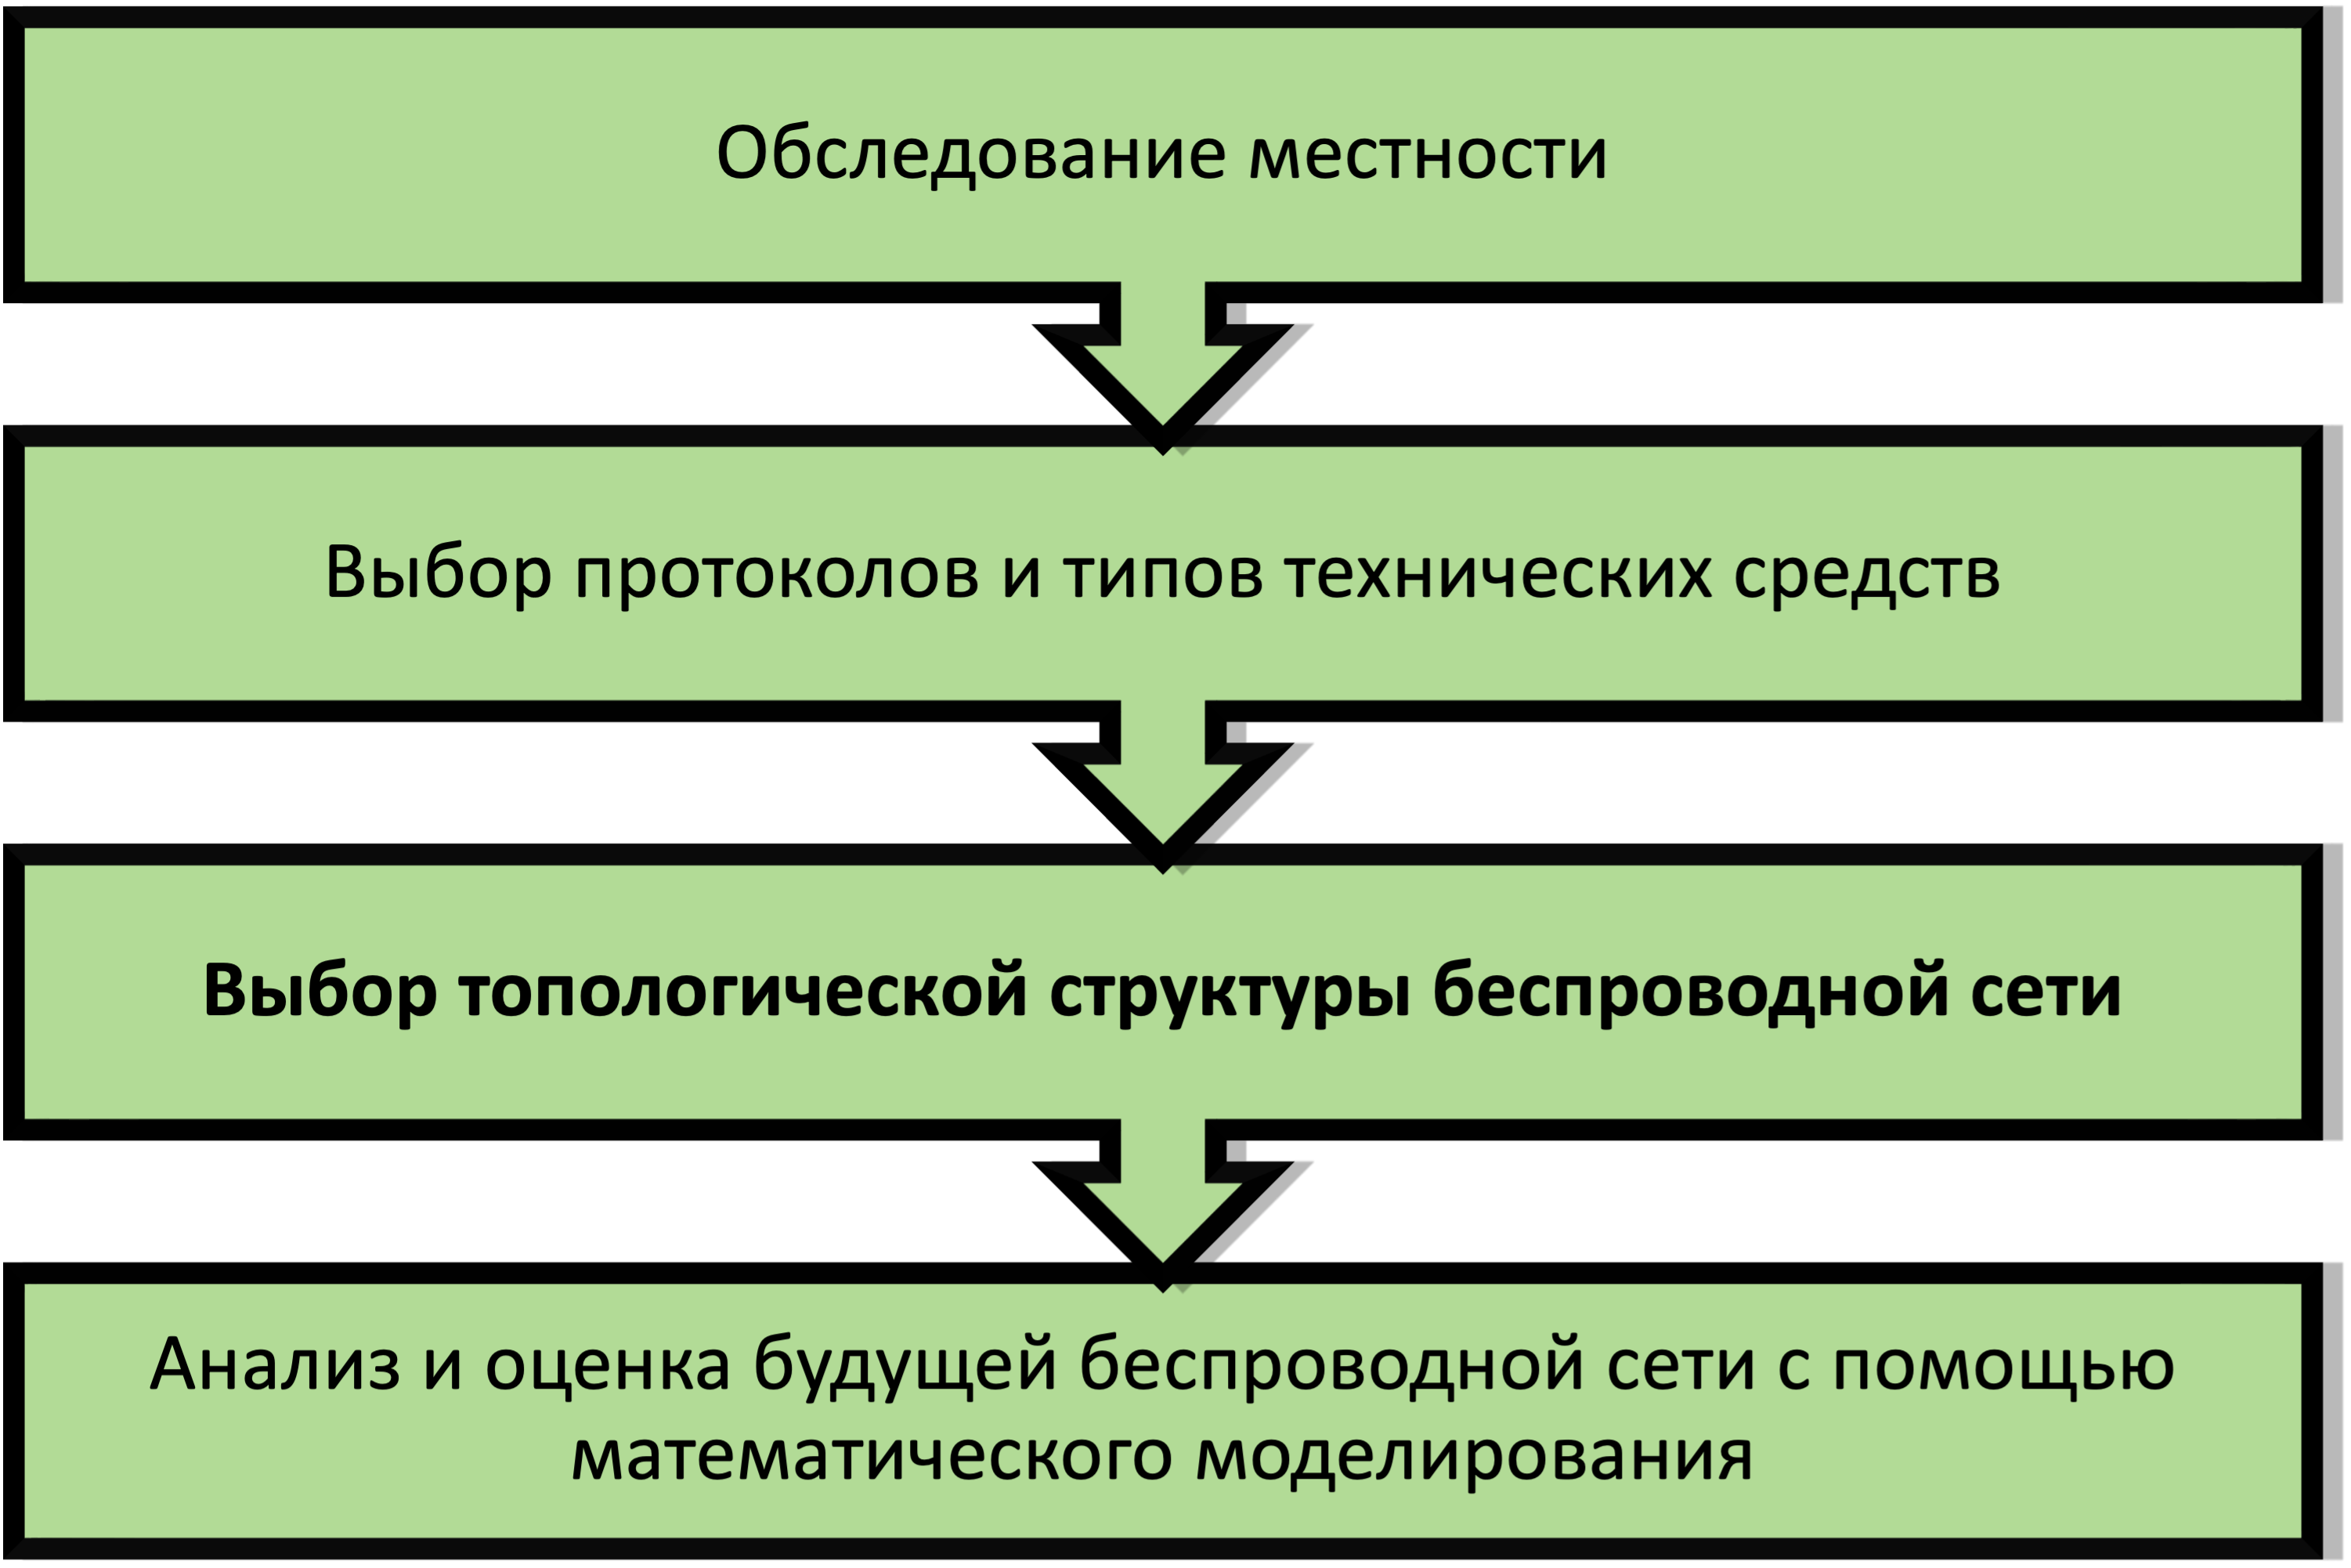
\includegraphics[width=0.65\textwidth]{design_stages.png}
  \caption{Этапы проектирования БШС.}
  \label{fig:part1_design_stages}
  \end{figure}


% В главе представлена методика расчета технологических параметров БШС, необходимых для решения задач размещения базовых станций. 

При развертывании сети необходимо обеспечить максимальное телекоммуникационное покрытие вдоль протяженной транспортной магистрали с условием обеспечения связи между шлюзами через систему размещенных БС БШС. В главе исследуются методы расчета дальности телекоммуникационной связи, необходимые в дальнейшем для р ешения задачи размещения БС. Рассмотрены распространенные на практике модели распространения радиосигналов: модель потери в свободном пространстве,  модель распространения SUI (Standford University Interim), модель двухлучевого распространения, модель Окамура-Хата. С помощью данных моделей распространения сигнала рассчитываются параметры задачи: радиус телекоммуникационной связи $ R_{jq}$ между базовыми станциями и радиус телекоммуникационного покрытия транспортной магистрали $ r_j $, необходимые для формулировки и решения задачи оптимального размещения базовых станций беспроводной сети. 


% Мощность принимаемой антенны рассчитывается из уравнения передачи Фрииса:

% \begin{displaymath}
% \label{eq:part3_Friis}
% \frac{P_{recv}}{P_{tr}} = G_{tr}G_{recv}\left(\frac{c}{4\pi R f} \right)^2,
% \end{displaymath}
% где
% $c$ --  скорость света,
% $f$ -- частота, 
% $R$ рассточние между приемной и передающей антенной.

% %   The Free Space Path Loss ($ FSPL $) equation defines the propagation signal loss between two antennas through free space (air):
% Исходя из параметров антенн на приемнике и передатчике возможно оценить максимальную потерю сигнала при распространении между двумя антеннами в свободном пространстве (в воздухе): $L_{fs}$:

% \begin{equation}
% \label{eq:part3_FSPL}
% FSPL = \left(\frac{4\pi R f}{c} \right)^2.
% \end{equation}

% Формула \cref{eq:part3_FSPL}, выраженная в децибеллах будет выражаться как

% \begin{equation}
% \label{eq:part3_L_fs}
% L_{fs} = 20 \lg{F} + 20\lg{R} + K,
% \end{equation}
% где $F$ -- центральная частота, на котором работает канал связи, $R$ -- расстоние между приемной и передающей антенной и $K$ -- константа, зависящая от размерностей частоты и расстояния:

% Дальность связи получаем из уравнений \cref{{eq:part3_link_budget}} и \cref{eq:part3_L_fs}:

% \begin{equation}
% \label{eq:part3_D}
% R = 10^{\left(\frac{L_{fs} - 20\lg{F} - K}{20}\right)}.
% \end{equation}

% Используя формулу \cref{eq:part3_D} можем расчитать теоретическую максимальную дальность связи $ R_{jq}$ между базовыми станциями и радиусом покрытия $ r_j $ с предположением об отсутствии препятствий, отражений, влияния контуров местности и т. д. Это допущение приемлемо для рассматриваемого случая с открытой местностью. Для расчета дальности связи $R_{jq}$, базовые станции $s_j$ и $s_q$ будут рассматриваться как станции \textit{передатчик} и \textit{приемник}, соответственно. Будем считать, что станции обрудованы направленными антеннами с усилениями $G_{tr}^{R}$ и $G_{recv}^{R}$. Каждая базовая станция оснащена всенаправленной антенной с чувствительностью $G_ {recv}^{r}$. Данная антенна необходимо для покрытия заданной области. При вычислении радиуса покрытия $r_j$ базовую станцию будем считать \textit{приемником}, а абонентсткое устройство \textit{передатчиком}.


% Одной из важных характеристик производительности сети является ее межконцевая задержка. В главе представлен аналитический метод расчета для БШС с линейной топологией и кросс-трафиком.

% Все БС связаны последовательно между собой в сеть с линейной топологией. Для расчета межконцевой задержки рассмотрим беспроводную сеть как сеть массового обслуживания (СеМО) с узлами $M/M/1$. В теории массового обслуживания , используя нотацию Кендалла узел СеМО описывается с использованием четрех факторов, записанных как $A / B/ n / m $ , где $A$ -- описывает входящий поток запросов; $B$ -- распределение времени обслуживания запросов; $n$ -- количество индентичных параллельных облуживающих устройств и $m$ -- длина буфера ожидания \cite{VishnevskyBook}. В случая отстутсвия описания $m$, считается, что $m = \infty$.
% % \begin{itemize}
% %     \item $A$ -- описывает входящий поток запросов;
% %     \item $B$ -- распределение времени обслуживания запросов;
% %     \item $n$ -- количество индентичных параллельных облуживающих устройств;
% %     \item $m$ -- длина буфера ожидания.
% % \end{itemize}
% % В случая отстутсвия описания $m$, считается, что $m = \infty$.

% Символом $M$ обозначают показельное распределение. В нашем случае узел $M/M/1$ характеризуется экспоненциальным распределнием интервалов между поступления пакетов, экспоненициальным распределением времени осблуживания и одним обслуживающим прибором. На каждый узел данной СеМО входящие потоки поступают с интесивностью $\lambda$. 

% По теореме Бурке \cite{Burke1956} на выходе узла $M/M/1$, а значит на входе каждой последующей фазы тоже пуассоновский поток. Интенсивность на выходе каждой фазы равна суммарной интенсивности всех входящих потоков с интенсивностями $\lambda$.

% По формуле Литтла \cite{Little1961} можно рассчитать время задержки на фазе. Интенсивность времени обслуживания рассчитывается по формуле: 

% \begin{displaymath}
%     \mu_j = p_j / w,
% \end{displaymath}
% где $p_j$ - пропускная спобоcтность $j$-ой станции, Мбит/с; $w$ - средний размер пакета, Мбит.

% Для каждой станции коэффициент загрузки равен:


% \begin{displaymath}
% \rho_j= \frac{\sum{\lambda}}{\mu_j} = \frac{q \cdot \lambda}{\mu_j} <1,
% \end{displaymath}
% где $q$ -- число входящих потоков. Условие $\rho_j<1$ является необходимым и достаточным условием существования стационарного режима функционирования СеМО.

% Тогда среднее время задержки по времени на каждой станции:

% \begin{displaymath}
%     \overline{T_j} = \frac{\rho_j}{1 - \rho_j} \cdot \frac{1}{q \cdot \lambda}.
% \end{displaymath}

% Межконцевая задержки в сети равна

% \begin{equation}
%     \label{eq:end_to_end_delay}
%     T^{e2e}= \sum{\overline{T_j}}.
% \end{equation}

При проектировании необходимо оценивать характеристики производительности БШС.
Одной из таких характеристик производительности сети является межконцевая задержка передачи пакетов в сети. В работе исследуются различные стохастические модели многофазной сети массового обслуживания (СеМО) с кросс-трафиком, экспоненциальным распределением интервалов между поступлениями пакетов и различными распределениями времени обслуживания. Рассмотрены модели многофазной СеМО: с узлами $M/M/1/N$ -- с экспоненциальным распределением времени обслуживания и конечным размером буфера, с узлами $M/PH/1/N$ -- с фазовым распределением времени обслуживания и конечным размером буфера. Такие модели труднорешаемы, точный аналитический расчет может быть невозможен из-за экспоненциального роста сложности решения с ростом числа фаз в сети.   Для оценки времени задержки для сетей с большим числом фаз прибегают к методу Монте-Карло. Также исследовалась простейшая модель СеМО с узлами $M/M/1$, для которой существует аналитическое решение. Модели сравнивались с временными задержками, полученными с помощью имитационного моделирования в среде NS-3 для БШС протокола IEEE 802.11n. Сравнение моделей представлено на рисунке \cref{fig:comparison_queue_models}. Как видно из графиков СеМО с узлами $M/M/1$ показывает достаточное приближение к данным имитационного моделирования. С учетом быстрого аналитического решения и достаточного приближения для оценки величины межконцевой задержки в ходе поиска оптимального размещения БС БШС было решено в работе использовать СеМО с узлами $M/M/1$ и кросс-трафиком.


% В главе представлен аналитический метод расчета задержек для БШС с линейной топологией и кросс-трафиком с помощью модели СеМО с узлами $M/M/1$. В дальнейшем данный метод расчета будет необходим для оценки задержек при решении задачи поиска оптимального размещения БС.



% Исследование таких СеМО представлено автором в работе \cite{Larionov2021}, в которой предложен метод калибровки моделей массового обслуживания с помощью имитационного моделирования в среде NS-3 БШС протокола IEEE 802.11n. На вход поступали пакеты, сгенерированные по экспоненциальному закону. С помощью NS-3 была получена выборка, для которой было восстановлено PH-распределения по трем моментам для случая с узлами $M/PH/1/N$ и экспоненциальное распределение по среднему значению для случая с узлами $M/M/1/N$. Также представлена модель $M/M/1$ с бесконечным буфером. Сравнение моделей представлено на рисунке \cref{fig:comparison_queue_models}. Как видно из графиков СеМО с узлами $M/M/1$ показывает достаточное приближение. В главе представлен аналитический метод расчета задержек для БШС с линейной топологией и кросс-трафиком с помощью модели СеМО с узлами $M/M/1$. В дальнейшем данный метод расчета будет необходим для оценки задержек при решении задачи поиска оптимального размещения БС.

\begin{figure}[h!]
  \centering
   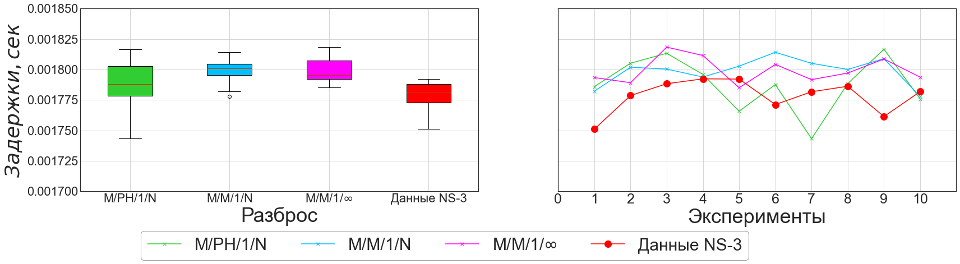
\includegraphics[width=1\textwidth]{comparison_queue_models.png}
\caption{Сравнение моделей массового обслуживания с данным NS-3}
\label{fig:comparison_queue_models}
\end{figure}




\FloatBarrier
\underline{\textbf{Вторая глава}} посвящена задаче оптимального размещения БС БШС для телекоммуникационного покрытия протяженной транспортной магистрали. Примерами протяженных магистралей могут являться: автомобильные и железные дороги, тоннели метрополитена, магистральные нефте- и газопроводы. Проблема формулируется в виде задачи целочисленного линейного программирования (ЦЛП) и в виде комбинаторной модели в экстремальной форме. 

Задан отрезок вдоль протяженной магистрали длиной $L$ с концами в точках $a_0$ и $a_{n+1}$. Внутри  отрезка $[a_0, a_{n+1}]$ задано конечное множество точек размещения $A=\{a_i\}, i=\overline{1,n}$. Каждая точка $a_i$ определяется своей одномерной координатой $l_i$. Заданы БС специального вида $s_{m+1}$ -- шлюзы. Шлюзы размещены на концах $a_0$ и $a_{n+1}$ отрезка.

\textbf{Задача в виде ЦЛП} формулируется следующим образом. Для того чтобы максимизировать телекоммуникационное покрытие вдоль протяженной транспортной магистрали необходимо разместить БС с учетом ограничением на суммарную стоимость размещаемых БС. Важно обеспечить связь любой станции со шлюзами на концах участка через систему размещаемых БС. 

Задано множество станций $S = \{s_j\}$. Каждой станции приписаны параметры $s_j = \{r_j, \{R_{jq}\}, c_j \}$, $j = \overline{1,m}; q = \overline{1,m}; q \neq j$. Здесь $r_j$ -- радиус покрытия станции, $R_{jq}$ -- это радиус связи между станциями $s_j$ и $s_q$, $c_j$ -- стоимость.  Для шлюзов радиуса покрытия $r_{m+1}=0$, радиус связи и стоимость не заданы. Задано стоимостное ограничение $C$.  

Целевая функция задачи:
\begin{equation}
    \label{eq:part3_objective_function}
    f =  \sum\limits_{i=1}^n (y_i^- + y_i^+) \rightarrow max,
  \end{equation}
где $y_i^+$ и $y_i^-$, $i= \overline{0,n+1}$ определяют охват покрытия (справа и слева, соответственно) станций.

% Перейдем к ограничениям задачи.

Введем двоичные переменные $x_{ij}$. Тогда $x_{ij}=1$, если станция $s_j$, размещенная на точке $a_i$, и $x_{ij}=0$, в противном случае; $i= \overline{1, n}$; $j = \overline{1,m}$. Введем двоичные переменные $ e_i $. Тогда $ e_i = 1 $, если какая-либо станция находится в точке $ a_i $, и $ e_i = 0$,  в противном случае; $ i = \overline {1, n} $. Для точек размещения шлюзов $ a_0 $ и $a_{n + 1}$ переменные $ e_0 = 1 $ и $ e_{n + 1} =1 $, соответственно.

% По определению \cref{eq:part3_ei}:



Каждая станция должна быть размещена только в одной точке \cref{eq:part3_ei, eq:part3_xij}:

\begin{equation}
    \label{eq:part3_ei}
    e_i =  \sum\limits_{j=1}^m x_{ij}, \quad i = \overline{1,n},
  \end{equation}

\begin{equation}
  \label{eq:part3_xij}
  \sum\limits_{i=1}^n x_{ij} \leq 1, \quad j = \overline{1,m}. 
\end{equation}

Значения покрытий не превышают радиус покрытия $r_j$ станции, размещенной в точке $ a_i $, и равны 0, если в точке $a_i$  нет станции \cref{eq:part3_yi_1, eq:part3_yi_2}:

\begin{equation}
  \label{eq:part3_yi_1}
  y_i^+ \leq \sum\limits_{j=1}^m x_{ij} \cdot r_j, \quad i = \overline{1,n};
\end{equation}

\begin{equation}
  \label{eq:part3_yi_2}
  y_i^- \leq \sum\limits_{j=1}^m x_{ij} \cdot r_j, \quad i = \overline{1,n}. 
\end{equation}

Общая область покрытия между любыми двумя точками $ a_i $ и $ a_k $, где расположены станции, не может превышать расстояние между этими точками \cref{eq:part3_yi_3, eq:part3_yi_4}.

\begin{equation}
  \label{eq:part3_yi_3}
  y_i^+ + y_k^- \leq \frac{l_k - l_i}{2} \cdot (e_i + e_k ) + (2 - e_i - e_k ) \cdot L, \quad i = \overline{1,n},  \quad k = \overline{i+1,n+1};
\end{equation}

\begin{equation}
  \label{eq:part3_yi_4}
  y_i^- + y_k^+  \leq \frac{l_i-l_k}{2} \cdot (e_i + e_k) + (2 - e_i - e_k) \cdot L, \quad i = \overline{1,n}, \quad k = \overline{i-1,0},
\end{equation}
где $ l_k $ и $ l_i $ - координаты точек $ a_i $ и $ a_k $, соответственно. 
% Это условие исключает влияние пересечений покрытий станций при вычислении общего значения покрытия между станциями.

% Согласно условиям задачи, станция, расположенная в $ a_i $, должна быть связана хотя бы с одной станцией слева и одной станцией справа, включая станции на конечных точках $ a_0 $ и $a_{n + 1}$. 

Введем бинарные переменные $z_{ijkq}, i = \overline{0,n}; j= \overline{1,m+1}; k=\overline{0,n},  k \neq i; q= \overline{1,m+1}, q \neq j$. Переменная $ z_ {ijkq} = 1$, если в точке $ a_i $ размещена БС $ s_j $ и данная БС связана с БС $ s_q $, размещенной в точке $ a_k $; и $ z_ {ijkq} = 0 $, в противном случае.
%
% Переменная $ z_{ij0(m + 1)} = 1$, если БС $ s_j $, размещенная в точке $ a_i $, связана со шлюзом $ s_{m + 1} $ в точке $ a_0 $; $ z_{ij0 (m + 1)} = 0 $ в противном случае. Переменная $ z_{ij(n + 1)(m + 1)} = 1 $, если БС $ s_j $, размещенная в точке $ a_i $, связана со шлюзом $ s_{m + 1} $ в точке $ a_{n + 1} $; $ z_{ij0(m + 1)} = 0 $  в противном случае.

% Введем бинарные переменные $z_{ijkq}, i = \overline{1,n}; j= \overline{1,m}; k=\overline{1,n},  k \neq i; q= \overline{1,m}, q \neq j$. Переменная $ z_ {ijkq} = 1$, если в точке $ a_i $ размещена БС $ s_j $ и данная БС связана с БС $ s_q $, размещенной в точке $ a_k $; и $ z_ {ijkq} = 0 $ в противном случае.
% Переменная $ z_{ij0(m + 1)} = 1$, если БС $ s_j $, размещенная в точке $ a_i $, связана со шлюзом $ s_{m + 1} $ в точке $ a_0 $; $ z_{ij0 (m + 1)} = 0 $ в противном случае. Переменная $ z_{ij(n + 1)(m + 1)} = 1 $, если БС $ s_j $, размещенная в точке $ a_i $, связана со шлюзом $ s_{m + 1} $ в точке $ a_{n + 1} $; $ z_{ij0(m + 1)} = 0 $  в противном случае.

% Станции должны быть размещены в обеих точках $ a_i $ и $ a_k $, \cref{eq:part3_z_ijkq_1, eq:part3_z_ijkq_2}:

\begin{equation}
  \label{eq:part3_z_ijkq_1}
  z_{ijkq} \leq e_i , \quad i = \overline{1, n}; \quad j = \overline{1, m}; \quad k = \overline{1,n}, k \neq i; \quad q = \overline{1,m}, q \neq j;
\end{equation}


\begin{equation}
  \label{eq:part3_z_ijkq_2}
  z_{ijkq} \leq e_k , \quad k = \overline{1, n}; \quad j = \overline{1, m}; \quad i = \overline{1,n}, i \neq k; \quad q = \overline{1,m}, q \neq j.
\end{equation}

% \fixme{====================================}

% Необходимо обеспечить коммуникационную связь справа от БС \cref{eq:part3_z_ijkq_1_1, eq:part3_z_ijkq_1_2}. Станция $ s_j $ в точке $ a_i $ должна быть связана с  любой станцией, расположенной в точке $ a_k $, справа от $ a_i $ ($ k> i $) или с правым шлюзом $ s_{m + 1} $ \cref{eq:part3_z_ijkq_1_1} 

\begin{equation}
  \label{eq:part3_z_ijkq_1_1}
  \sum\limits_{k=i+1}^{n} \sum\limits_{\substack{q = 1\\ q \neq j}}^m z_{ijkq} + z_{ij(n+1)(m+1)} = x_{ij} ,  \quad i = \overline{1, n}, \quad j = \overline{1, m}.
\end{equation}
% Требуется чтобы станция, размещенная справа от $s_j$ или правый шлюз $ s_{m + 1} $  были связаны с размещаемой станцией $ s_j $ \cref{eq:part3_z_ijkq_1_2}

\begin{equation}
  \label{eq:part3_z_ijkq_1_2}
  \sum\limits_{k=i+1}^{n} \sum\limits_{\substack{q = 1\\ q \neq j}}^m z_{kqij} + z_{(n+1)(m+1)ij} = x_{ij} ,  \quad i = \overline{1, n}, \quad j = \overline{1, m}.
\end{equation}

% Необходимо обеспечить коммуникационную связь слева от БС \cref{eq:part3_z_ijkq_2_1, eq:part3_z_ijkq_2_2}. Станция $ s_j $ в точке $ a_i $ должна быть связана с  любой станцией, расположенной в точке $ a_k $, слева от точки $ a_i $ ($ k <i $) или с левым шлюзом $ s_{0}$ \cref{eq:part3_z_ijkq_2_1} 

\begin{equation}
  \label{eq:part3_z_ijkq_2_1}
  z_{ij0(m+1)} + \sum\limits_{k=1}^{i-1} \sum\limits_{\substack{q = 1\\ q \neq j}}^m z_{ijkq}= x_{ij}, \quad i = \overline{1, n}, \quad j = \overline{1, m}.
\end{equation}
% Требуется чтобы станция, размещенная слева от $s_j$ или левый шлюз $ s_{0} $  были связаны с размещаемой станцией $ s_j $ \cref{eq:part3_z_ijkq_2_2}

\begin{equation}
  \label{eq:part3_z_ijkq_2_2}
    z_{0(m+1)ij} +  \sum\limits_{k=1}^{i-1} \sum\limits_{\substack{q = 1 \\ q \neq j}}^m z_{kqij}= x_{ij},  \quad i = \overline{1, n}, \quad j = \overline{1, m}.
\end{equation}


% \fixme{===================================}

% Необходимо, чтобы станция $ s_j $ в точке $ a_i $ была связана с  любой станцией, расположенной в точке $ a_k $, справа от $ a_i $ ($ k> i $) или с правым шлюзом $ s_{m + 1} $, \cref{eq:part3_z_ijkq_3_1, eq:part3_z_ijkq_3_2}. 

% \begin{equation}
%   \label{eq:part3_z_ijkq_3_1}
%   \sum\limits_{k=i+1}^{n} \sum\limits_{\substack{q = 1\\ q \neq j}}^m z_{ijkq} + z_{ij(n+1)(m+1)} = x_{ij} ,  \quad i = \overline{1, n}, \quad j = \overline{1, m}.
% \end{equation}

% Станция $ s_j $, размещенная в $ a_{n} $, справа связана толко со шлюзом $ s_{m + 1} $ на месте $ a_ {n+1}$ \cref{eq:part3_z_ijkq_3_2}. 


% \begin{equation}
%   \label{eq:part3_z_ijkq_3_2}
%   z_{nj(n+1)(m+1)} = x_{nj} \quad j = \overline{1, m}.
% \end{equation}

% Также станция должна быть связана с любой станцией, расположенной в точке $ a_k $ слева от точки $ a_i $ ($ k <i $) или с левым шлюзом $ s_{m + 1} $, \cref{eq:part3_z_ijkq_4_1, eq:part3_z_ijkq_4_2}.

% \begin{equation}
%   \label{eq:part3_z_ijkq_4_1}
%   z_{1j0(m+1)}= x_{ij}, \quad j = \overline{1, m}.
% \end{equation}

% Станция $s_j$, размещенная в точке $a_{1}$ слева может быть связана только со шлюзом $s_{m+1}$, расположенном в точке $a_0$ \cref{eq:part3_z_ijkq_4_1}.

% \begin{equation}
%   \label{eq:part3_z_ijkq_4_2}
%   z_{ij0(m+1)} + \sum\limits_{k=1}^{i-1} \sum\limits_{\substack{q = 1\\ q \neq j}} z_{ijkq}= x_{ij}, \quad i = \overline{2, n}, \quad j = \overline{1, m}.
% \end{equation}

% Необходимо, чтобы станция $ s_q $ в точке $ a_k $ была связана с любой станцией справа, расположенной в точке $ a_i $ \cref{eq:part3_z_ijkq_5}.

% \begin{equation}
%   \label{eq:part3_z_ijkq_5}
%   \sum\limits_{i=k+1}^{n} \sum\limits_{\substack{j=1 \\ j \neq q}}^m z_{ijkq} = x_{kq} , \quad k = \overline{1, n-1}, \quad q = \overline{1, m}.
% \end{equation}

% Кроме того, станция $ s_q $ в точке $ a_k $ подключена к любой станции слева, расположенной в точке $ a_i $ \cref{eq:part3_z_ijkq_6}. 


% \begin{equation}
%   \label{eq:part3_z_ijkq_6}
%   \sum\limits_{i=1}^{k} \sum\limits_{\substack{j=1 \\ j \neq q}}^m z_{ijkq} = x_{kq} , \quad k = \overline{2, n}, \quad q = \overline{1, m}.
% \end{equation}

% \fixme{===================================}

Неравенства \cref{eq:part3_z_ijkq_1, eq:part3_z_ijkq_2} и равенства \cref{eq:part3_z_ijkq_1_1, eq:part3_z_ijkq_1_2, eq:part3_z_ijkq_2_1, eq:part3_z_ijkq_2_2} обеспечивают условие симметрии связи между базовыми станциями, расположенными в точках $ a_i $ и $ a_k $, $\forall i, k $. 


Если станции $ s_j $ и $ s_q $ связаны, то их радиусы связи должны быть не меньше расстояния между точками $ a_i $ и $ a_k $, где расположены станции \cref{eq:part3_z_ijkq_7, eq:part3_z_ijkq_8}.

\begin{equation}
    \begin{gathered}
  \label{eq:part3_z_ijkq_7}
  z_{ijkq}(R_{jq}-(a_i-a_k ))\geq 0, \\i= \overline{1,n}; \quad k=\overline{0,i-1}; \quad j=\overline{1,m}; \quad q= \overline{1,m}, q \neq j; 
    \end{gathered}
\end{equation}

\begin{equation}
    \begin{gathered}
  \label{eq:part3_z_ijkq_8}
  z_{ijkq} (R_{jq}-(a_k-a_i )) \geq 0,  \\ i= \overline{1,n}; \quad k=\overline{i+1,n+1};  \quad j=\overline{1,m}; \quad q= \overline{1,m}, q \neq j.
    \end{gathered}
\end{equation}

И ограничение на стоимость размещаемых станций

\begin{equation}
  \label{eq:part3_cost}
  \sum\limits_{i=1}^n \sum\limits_{j=1}^m x_{ij} \cdot c_j \leq C,
\end{equation}
где $c_j$ -- стоимость БС $s_j$.



Для частного случая в работе \cite{Ivanov2018}, где размещаются множество однотипных станций вдоль протяженной магистрали, представлено доказательство NP-трудности задачи. Так как математическая модель \cref{eq:part3_objective_function, eq:part3_ei, eq:part3_xij, eq:part3_yi_1, eq:part3_yi_2, eq:part3_yi_3, eq:part3_yi_4, eq:part3_z_ijkq_1, eq:part3_z_ijkq_2, eq:part3_z_ijkq_1_1, eq:part3_z_ijkq_1_2, eq:part3_z_ijkq_2_1, eq:part3_z_ijkq_2_2, eq:part3_z_ijkq_7, eq:part3_z_ijkq_8, eq:part3_cost} является обобщением указанной задачи, в которой размещаются множество БС с различными параметрами, она также является NP-трудной. Модель ЦЛП рассчитывалась в пакете Optimization Toolbox MATLAB.

% Была получена математическая модель в виде задачи целлочисленного-линейного программирования \cref{eq:part3_objective_function, eq:part3_xij, eq:part3_yi_1, eq:part3_yi_2, eq:part3_yi_3, eq:part3_yi_4, eq:part3_z_ijkq_1, eq:part3_z_ijkq_2, eq:part3_z_ijkq_3_1, eq:part3_z_ijkq_3_2, eq:part3_z_ijkq_4_1, eq:part3_z_ijkq_4_2, eq:part3_z_ijkq_5, eq:part3_z_ijkq_6, eq:part3_z_ijkq_7, eq:part3_z_ijkq_8, eq:part3_cost, eq:syn_ilp_y, eq:syn_ilp_x, eq:syn_ilp_z}. Для частного случая, представленного в работе \cite{Ivanov2018}, где размещаются множество однотипных станций вдоль линейного участка, было представлено докозательнство NP-полноты. Данная модель является обощением частного случая, следовательно также является NP-полной. Модель ЦЛП рассчитывалась в пакете Optimization Toolbox MATLAB.
%  усовершенствованным алгоритмом Лэнд и Дойг \cite{Land1960}. 

% Одной из важных характеристик производительности сети является ее межконцевая задержка. Необходимо оценивать характеристику и использовать ее в качестве ограничения при синтезе топологической структуры сети. Представить данное ограничение в линейной форме для модели ЦЛП невозможно. 
% Для учета данного ограничения в работе разработана комбинаторная модель в экстремальной форме и алгоритм специального вида на методе ветвей и границ.

Использование программных пакетов для расчета задачи в виде ЦЛП в каноническом виде не учитывает специфику задачи, а следовательно, решает исследуемую задачу не самым эффективным способом. Кроме того, при решении задачи синтеза топологии интересно было бы учитывать характеристики производительности БШС, например среднюю межконцевую задержку. Для того чтобы учесть специфику задачи, а именно размещение БС с обеспечением наличия связи между ними и ограничение величины задержки в сети, в главе представлена комбинаторная модель в экстремальной форме задачи размещения БС БШС.


% \fixme{Написать посстановку}

% Одной из важных характеристик производительности сети является ее межконцевая задержка. Необходимо оценивать характеристику и использовать ее в качестве ограничения при синтезе топологической структуры сети. Представить данное ограничение в линейной форме для модели ЦЛП невозможно. 
% Для учета данного ограничения 

% В работе разработана комбинаторная модель в экстремальной форме и алгоритм специального вида на методе ветвей и границ. Помимо бюджетного ограничения существует необходимость учитывать также характеристики производительности БШС. Одной из таких характеристик является межконцевая задержка, которая будет учитываться как ограничение задачи.

\textbf{Задача в виде комбинаторной модели в экстремальной форме.} Сформулирована комбинаторная модель в экстремальной форме и разработан новый алгоритм ее решения, основанный на методе ветвей и границ (МВиГ). В формулировке задачи кроме стоимостного ограничения учитывается также ограничение на величину задержки передачи пакетов в сети $T$. Каждой станции $s$ множества $S$ приписаны параметры $s_j=\{r_j,\{R_{jq} \},p_j, c_j \},j=1,...,m;q=1,...,m;j \neq q $, где $r_j$ -- максимальный радиус покрытия БС, $\{R_{jq} \}$ -- матрица радиусов телекоммуникационной связи между $j$-ой и $q$-ой станциями, $p_j$ -- пропускная способность БС и $c_j$ -- стоимость.



% Для удовлетворения данного ограничения и снижения времени решения задачи в главе представлена постановка задачи и ее формулировка в специальной экстремальной комбинаторной форме.

\textit{Допустимой расстановкой станций} является возрастающий по величине координат $l_i$  набор пар $P = \{a_i, s_j\},a_i \in A,i \neq 0,i \neq n+1;s_j \in S$, для которого выполняются требования:

\begin{enumerate}
    \item  Для каждой пары $(a_i,s_j)$:
        \begin{enumerate}
            \item слева: либо найдется такая пара $(a_k,s_q)$, что, $l_i - l_k \leqslant R_{jq}$  и $l_i - l_k  \leqslant R_{qj}$, либо $l_i-l_0 \leqslant R_{j0}$ и $l_i - l_0 \leqslant R_{0j}$;
            \item справа: либо найдется такая пара $(a_t,s_g)$, что, $l_t-l_i \leqslant R_{jq}$ и $l_t - l_i \leqslant R_{qj}$, либо $l_{n+1}-l_i \leqslant R_{j(m+1)}$ и $l_{n+1}-l_i \leqslant R_{(m+1)j}$. 
        \end{enumerate}

Данное требование гарантирует, что любая станция может быть связана со станциями на концах отрезка либо через промежуточные станции, либо непосредственно.
    \item Сумма задержек по всем размещенным станциям меньше заданной величины $T$ – средней межконцевой задержки по времени по всей системе станций:
    \begin{displaymath}
        \label{eq:part3_e2e_delay}
        \sum\limits_{j \in S_\sigma} \overline{T_j} \leqslant T,
    \end{displaymath}
где $S_\sigma$ – множество размещенных станций, $\overline{T_j}$ -- среднее время задержки на станции. Расчет задержки проводится с помощью многофазной модели СеМО.
    \item Суммарная стоимость размещенных станций меньше заданного ограничения на стоимость $C$.
\end{enumerate}

Каждой допустимой расстановке станций $P$ соответствует величина покрытия $z(P)$, определяемая как суммарная область телекоммуникационного покрытия БС, входящих в набор пар $P$. Для удобства описания введем понятие <<недопокрытия>> $f(P)$:

\begin{equation}
    \label{synopsis_f(p)}
    f(P) = L - z(P).
\end{equation} 

\textbf{Задача 1.}
Пусть $G$ -- множество всех допустимых расстановок $P$.
Требуется найти такую допустимую расстановку  $P^*$, что
\begin{displaymath}
    P^* = \argmin \limits_{P \in G} f(P).
\end{displaymath}

% Обозначим через $\Gamma$ все множество вариантов размещения станций (не обязательно допустимых) из множества $S$ на заданном множестве возможных мест их размещения.


% Описываемая процедура использует известный прием разбиения множества $G$ на подмножества с использованием некоторого параметра. 
Пусть $\Gamma$ все множество вариантов размещения БС, необязательно допустимых. Представлена процедура построения бинарного дерева поиска для полного перебора без повторений всех элементов множества $\Gamma$. Процедура необходима для построения дерева поиска в алгоритме типа ветвей и границ. Пусть $G_0$ -- исходное множество $\Gamma$. На каждой итерации, начиная с $\nu=0$, текущее подмножество $G_\nu$ разбивается на два подмножества $G^1_\nu$ и $G^2_\nu$. При этом множество $G_\nu$ обычно называется «материнским», а множества $G^1_\nu$  и $G^2_\nu$  -- <<потомками>> множества $G_\nu$ или дочерними узлами.

% В множестве $S$ станции упорядочены по не убыванию радиусов покрытия. Процесс формирования и последовательность исследования подмножеств осуществляется с помощью дерева поиска,  где множеству $\Gamma$ соответствует корневая вершина.

% Обозначим через $\Gamma$ все множество вариантов размещения станций (не обязательно допустимых) из множества $S$ на заданном множестве возможных мест их размещения. В множестве $S$ станции упорядочены по не убыванию радиусов покрытия. Процесс формирования и последовательность исследования подмножеств осуществляется с помощью дерева поиска,  где множеству $\Gamma$ соответствует корневая вершина.



В качестве параметра разбиения используется переменная $\pi_{ij}$, принимающая два значения 0 и 1: $\pi_{ij}=1$, если наложено условие, что на месте $a_i$ расположена БС $s_j$; $\pi_{ij} = 0$, в противном случае.


Для построения алгоритма типа ветвей и границ разработаны методы исследования вершин дерева на возможность их закрытия. Возможны три случая: 1) доказано, что множество $G_\nu$ пусто, 2) доказано, что в множестве $G_\nu$ не может быть допустимой расстановки $P$ с меньшим значением целевой функции \cref{synopsis_f(p)}, чем у лучшей расстановки $\widehat{P}$ из уже найденных (рекорда), 3) найдено оптимальное решение на множестве $G_\nu$. На каждом узле дерева проводится оценка недопокрытия в виде суммы
 

% В соответствии с техникой МВиГ закрытие вершины в результате исследования, соответствующего ей множества $G_\nu$ возможно в трех случаях.

% \underline{\textit{\textbf{Случай 1.}}} Множество $G_\nu$ -- пусто, т.е. доказано, что в множестве $G_\nu$ при данном наборе фиксированных и запрещенных переменных $\pi_{ij}$ нет ни одной допустимой расстановки $P$.

% \underline{\textit{\textbf{Случай 2.}}} Доказано, что в множестве $G_\nu$ не может быть допустимой расстановки $P$ с меньшим значением целевой функции \cref{synopsis_f(p)}, чем у лучшей расстановки $\widehat{P}$ из уже найденных. Значение функции $f(\widehat{P})$ называется «рекордом», а расстановка $\widehat{P}$ -- «рекордным решением». В качестве начального рекорда принимается число заведомо большое искомого оптимального решения, например, $L$ – длина всего отрезка.

% \underline{\textit{\textbf{Случай 3.}}} Найдено оптимальное решение на множестве $G_\nu$.
% Прежде чем рассмотреть эти три случая, запишем важное свойство любого множеств $G_\nu$, являющееся следствием принятого правила выбора свободной переменной для разбиения очередного множества $G_\nu$ при прямом шаге.



\begin{displaymath}
    W\left(G_\nu\right) = w_1 + w_2. 
\end{displaymath}
Величина $w_1 \left(G_\nu \right)$ вычисляется как сумма всех частичных недопокрытий слева от точки размещения $a_k$ и величины радиуса покрытия, размещаемой БС. Оценка $w_2 \left(G_\nu \right)$ вычисляется для недопокрытия справа на части $\beta$ до конца всего отрезка (точки $a_{n+1}$). Оценка $w_1$ рассчитывается с помощью релаксацией условий, определяющих допустимую расстановку станций на участке $\beta$, в виде задачи булева программирования.

% Найдем такое подмножество $S_\beta$ множества станций $S$, состоящее из еще не размещенных станций и дающее минимальное «недопокрытие» на участке $\beta$ при выполнении только условий 2) – 4). Для этого сформулируем следующую задачу булева программирования.

\underline{\textit{\textbf{Задача 2.}}}
\begin{displaymath}
    z = |\beta| - \sum\limits_{x_j \in S_\beta} 2 \cdot r_j x_j \rightarrow min.
\end{displaymath}

\begin{equation}\label{eq:part4_task2_cost}
    \sum\limits_{x_j \in S_\beta} c_j x_j \leqslant C',
\end{equation}

\begin{equation}\label{eq:part4_task2_m}
    \sum\limits_{x_j \in S_\beta} x_j \leqslant m,
\end{equation}

\begin{displaymath}
    x_j \in \{0, 1\},
\end{displaymath}
где $|\beta|$ -- длина отрезка $\beta$, $m$ -- число свободных мест для размещения БС на отрезке $\beta$, $r_j$ -- радиус покрытия станции $s_j$, $c_j$ -- стоимость неразмещенных БС, $C'$ -- ограничение на стоимость с учетом уже размещенных БС.

% Очевидно, что эффективность использования оценки в методе ветвей и границ определяется точностью оценки и временем ее вычисления. \underline{\textit{\textbf{Задача 2}}} -- это задача ЦЛП, являющаяся труднорешаемой \cite{Gari}. На основании \underline{\textit{\textbf{задачи 2}}} можно получить две оценки менее точные, но имеющие более эффективные методы решения. Заметим, что при снятии ограничения \cref{eq:part4_task2_cost} или \cref{eq:part4_task2_m} \underline{\textit{\textbf{задача 2}}} представляет собой целочисленную задачу <<О ранце>> c эффективным псевдополиномиальным алгоритмом решения \cite{Gari}. При этом с точки зрения точности оценки, более перспективным представляется снятие ограничения \cref{eq:part4_task2_m}, так как на практике, обычно, число возможных мест размещения станций существенно меньше числа размещенных станций, полученного в результате решения задачи. 

Если множество $G_\nu$ получено из материнского множества добавлением условия $\pi_{kt}=0$, то оценка $W(G_\nu)$ равна оценке материнского множества. Если для найденной расстановки $P$ выполняются требования 1) –- 3) и

\begin{equation}
    \label{eq:part4_is_less_than_record}
    f(P) < f(\widehat{P}),
\end{equation}
то $f(P)$ принимается за новый рекорд $f(\widehat{P})$, расстановка $P$ становиться новым рекордным решением $\widehat{P}$ и далее выполняется шаг обратного хода по дереву поиска. Если неравенство \cref{eq:part4_is_less_than_record} не выполняется, то рекорд остается прежним и выполняется шаг обратного хода. Работа алгоритма типа ветвей и границ заканчивается, когда все вершины дерева поиска закрыты, при этом решение задачи 

\begin{displaymath}
    P^{*} = \widehat{P},  f(P^*) = f(\widehat{P}).
\end{displaymath}




% Был проведено численное сравнение двух моделей для частного случая с однотипными станциями и без учета ограничения на время доставки пакетов в сети. В задаче требовалось разместить весь набор $m$ имеющихся станций. Множество всех возможных вариантов комбинаций $m$ станций на  $n$ местах (не только допустимых) запишем как $\Gamma$. Общее количество $\gamma \in \Gamma$:

% \begin{displaymath}
% \gamma = C_n^m \times m!.
% \end{displaymath} 
%  В качестве характеристики сравнения двух методов было выбрано количество пройденных узлов в ходе поиска оптимального значения, чтобы параметры выполнения алгоритмов не зависели от скорости машины и/или качества реализации программного кода данных алгоритмов. В таблице \cref{tab:problems_BF_BnB_ILP} показаны результаты решения задач для различного числа количества размещения и количества станций с использованием полного перебора, алгоритма МВиГ и модели ЦЛП. Для каждого набора станций и набора размещений были рассчитаны 10 примеров с различными числовыми входными данными. Для <<$-$>> решение задачи данной размерности методом полного перебора не было получено за 3 ч счета. 
% Как видно из результов, представленных в таблице, при увеличении размерностей задачи, алгоритм МВиГ позволяет найти решение быстрее в ходе движения по дереву поиска.

% \begin{table}[b]\centering
%     \caption{Результаты численного решения.}\label{tab:problems_BF_BnB_ILP}
%     \begin{tabular}{|l|l|l|l|l|}
%     \hline
%     \textbf{Места} & \textbf{Станции} &	\textbf{Полный}& \textbf{МВиГ} & \textbf{ЦЛП} \\ 
%     \textbf{размещения} &  &	\textbf{перебор}&  &  \\
%     \hline
%     7 &		5 &	17550  &	933 &		\textbf{753}\\
%     9 &		5 &	71090  &	6478 &		\textbf{2669}\\
%     10 &	5 &	126180 &	\textbf{1041} &		8551\\
%     12 &	6 &	-- &		\textbf{8294} &		38569\\
%     13 & 	6 &	-- &		\textbf{18485} &	30369\\
%     \hline
%     \end{tabular}
% \end{table}
    

\textbf{Построение последовательности топологий для итерационной процедуры моделирования БШС.}
При проектировании БШС бывают ситуации, когда решение задачи размещения на этапе синтеза топологии не отвечает всем требованиям проектировщиков. На следующем этапе моделирования сети полученное размещение не удовлетворяет критериям данного этапа. Для решения этой проблемы разработан метод построения последовательности топологий для итерационной процедуры моделирования БШС, основанный на идее метода построения последовательности планов \cite{Emelichev}.



% При проектировании БШС надо найти ее оптимальную топологию среди всех топологий, для которых будут выполняться все требования к показателям, исследуемым и рассчитываемым на этапе моделировании сети. Для решения этой задачи воспользуемся идеей метода построения последовательности планов \cite{Emelichev}.

Для \textbf{задачи 1.} требуется найти такую допустимую расстановку $P^*$, что

\begin{displaymath}
    f(P^*) = min \{f(P), P \in G \}.
\end{displaymath}
Последовательность $\Gamma' = P^1, P^2, ... ,P^k$ допустимых расстановок множества $G$ для заданного $k$ выглядит следующим образом 
\begin{align}
    f(P^1) &= f(P^*), \nonumber  \\
    f(P^2) &= extr\{ f(P), P \in G \textbackslash P^1 \}, \nonumber \\
    ... \nonumber \\
    f(P^k) &= extr\{ f(P), P \in G \textbackslash P^1 \cup P^2 \cup ... P^k \}.
\end{align}
В последовательности $\Gamma'$ каждое решение не лучше предыдущего и не хуже последующего. Начиная с первой расстановки, полученной на этапе синтеза, будет выполняться следующий этап проектирования -- моделирования БШС. Как только будет получена расстановка, отвечающая всем требованиям проектировщиков, будет получено решение задачи нахождения оптимальной топологии среди всех найденных топологий.

Для поиска последовательности  $\Gamma'$ с помощью разработанного алгоритма необходимо заменить строгое неравенство \cref{eq:part4_is_less_than_record} следующим неравенством 

% Будем последовательно, начиная с первой расстановки, выполнять этап моделирования БШС. Как только будет получена расстановка, удовлетворяющая всем требованиям, будет получено решение задачи нахождения оптимальной топологии среди всех топологий, для которых выполняются все требования к характеристикам, исследуемым и рассчитываемым на этапе математического моделировании сети. Действительно, для всех предыдущих расстановок эти условия не выполняются, а все последующие расстановки в последовательности $\Gamma$ не могут быть лучше по критерию $f(P)$.

% Заменив неравенство \cref{eq:part4_is_less_than_record} на нестрогое и записывая все рекорды, полученные в процессе работы алгоритма можно получить последовательность расстановок, в которой каждая расстановка не хуже предыдущей и не лучше последующей. Для получения последовательности $\Gamma$ достаточно «перевернуть» полученную последовательность, где первый элемент станет последним.

% Недостатком такой процедуры является то, что для исследования на этапе моделирования будут отобраны только расстановки не хуже первого рекорда и среди них может не оказаться расстановки, удовлетворяющей критериям моделирования на следующих этапах.
% Для расширения множества $\Gamma$ можно сделать следующее. Зададим условие, что в результате решения \textbf{задачи 1} мы хотим получить не только оптимальное решение, но и все решения не хуже оптимального на величину $d$. Для решения такого варианта задачи достаточно неравенство \cref{eq:part4_is_less_than_record} в алгоритме МВиГ заменить следующим неравенством 

\begin{equation}
    \label{eq:part4_is_less_than_record_d}
    f(P) \leqslant f(\widehat{P}) + d,
\end{equation}
где $d = \varepsilon \cdot L > 0, \varepsilon$ -- заданное отклонение в процентах.

 
После нахождения оптимального размещения, с помощью алгоритма можно получить последовательность допустимых размещений, с недопокрытием $f(P)$ не более чем $d$ от оптимального.  На основании неравенства \cref{eq:part4_is_less_than_record_d} строится последовательность топологий для итерационной процедуры моделирования. Предложенный алгоритм и комбинаторная модель реализованы на языке Python.

% , увеличивая величину $d$, если при данном ее значении допустимого решения на этапе моделирования не найдено. Предложенный алгоритм и комбинаторная модель реализованы на языке Python.

% В работе представлено численное сравнение решения комбинаторной задачи с помощью разработанного алгоритма и решения модели в виде ЦЛП. Рассматривается частный случай с однотипными станциями и без учета ограничения на время доставки пакетов в сети. Результат сравнения говорит о целесообразности использования алгоритма при больших размерностях задачи.

% Обе задачи, в виде ЦЛП и в виде комбинаторной модели в экстремальной форме относятся к широкому к классу задач размещения мощностей. Отличительной особенностью рассмотренных задач является наличие условия на связь между размещаемыми объектами (базовыми станциями) и линейная контролируемая территория.

\underline{\textbf{В третьей главе}} сформулирована и решена задача оптимального размещения базовых станций для обслуживания заданного множества рассредоточенных объектов в виде задачи частично целочисленного линейного программирования (ЧЦЛП). Если во второй главе рассмотрена задача максимального телекоммуникационного покрытия, в третьей главе рассматривается постановка задачи минимизации суммарной стоимости, где необходимым условием является обеспечения телекоммуникационной связью всех заданных стационарных объектов.
Постановка представлена в общем случае, когда объекты размещены не только вдоль линейного участка, а рассредоточены на плоскости. Исследована модель потоковой задачи для проверки допустимости существования потока от объектов до шлюза. Предложена задача оптимального размещения БС, принадлежащая к широкому классу задач размещения мощностей (Location Allocation Problem). В рамках широкого класса задач размещения мощностей в данных задачах размещения присутствуют специфика на связь между всеми узлами сети.

% посвящена исследованию оптимального размещения БС БШС с ячеистой топологии. В предыдущей главе представлены модели и алгоритм для решения задачи максимального телекоммуникационного покрытия вдоль всей протяженной магистрали. На практике бывают задачи, когда покрытие всей протяженной магистрали не так существенно, как обеспечение телекоммуникационной связью  рассредоточенных стационарных объектов для передачи данных. В главе представлена математическая модель минимизации стоимости размещения БС БШС для обслуживания множества рассредоточенных объектов. Постановка представлена в общем случае, когда объекты размещены не только вдоль протяженной магистрали, а рассредоточены на плоскости. Задача относится к классу задач размещения мощностей с условием наличия телекоммуникационной связи между станциями.

% Задано множество вершин $A= \left\{ a_i \right\}, i=\overline{0,n}$ на плоскости. Каждая вершина $a_i$ имеет координаты $\left\{ x_i, y_i \right\}$.

% Множество $A$ состоит из двух подмножеств:
% \begin{itemize}
%     \item $A_1$ -- множество вершин, которое соответствует объектам, с которых необходимо собирать информацию. Каждой вершине $a_i$ приписана величина $v_i$.
%     \item $A_2$ -- множество мест, где размещены базовые станции. В дальнейшем вершину из $A_2$ будем идентифицировать  не только как место размещения, но и как соответствующую станцию.
% \end{itemize}

% По определению:
% $$
% A_1 \cup A_2 = \varnothing;
% $$

% $$
% A_1 \cap A_2 = A.
% $$

% Все вершины пронумерованы так,что:
% $$
% A_1 = \left\{a_i \right\}, i= \overline{1,n_1};
% $$

% $$
% A_2 = \left\{ a_i  \right\}, i= \overline{n_1+1,n}.
% $$

% Постановка задачи

% Задано множество вершин $A = a_i$, $i=\overline{0,n}$ на плоскости. Каждая вершина $a_i$ имеет координаты $\left\{ x_i, y_i \right\}$.
% Множество $A$ состоит из двух подмножеств: 
% \begin{itemize}
%     \item $A_1$ -- множество вершин, с которых необходимо собирать информацию. Каждой вершине $a_i$ приписана   величина $v_i$ -- максимальный объем информации, снимаемой с объекта, расположенного на этой вершине;
%     \item $A_2$ -- множество возможных мест размещения базовых станций. 
% \end{itemize}

% По определению

% $$
% A_1 \cup A_2 = \varnothing;
% $$

% $$
% A_1 \cap A_2 = A.
% $$

% Все вершины пронумерованы так, что $
% A_1 = \left\{a_i \right\}, i= \overline{1,n_1};
% $ и $
% A_2 = \left\{ a_i  \right\}, i= \overline{n_1+1,n}.
% $


% Задано множество типов базовых станций $S = s_j$, $j=\overline{1,m}$, которые необходимо разместить на множестве $A_2$. Каждой станции приписаны четыре параметра $s_j = \left\{r_j, R_{ij}, \vartheta_j, c_j \right\}$, где:
% $r_j$ -- максимальный радиус покрытия; $R_{ij}$ -- максимальный радиус связи между $i$-ой и $j$-ой станциями. Параметр характеризует расстояние, на котором обеспечивается связь между станциями; $\vartheta_j$ -- максимальный объем информации в единицу времени, который может быть получен от объектов, обслуживаемых данной станцией; $c_j$ -- стоимость станции.

% \begin{itemize}
%     \item $r_j$ -- максимальный радиус покрытия;
%     \item $R_{ij}$ -- максимальный радиус связи между $i$-ой и $j$-ой станциями. Параметр характеризует расстояние, на котором обеспечивается связь между станциями;
%     \item $\vartheta_j$ -- максимальный объем информации в единицу времени, который может быть получен от объектов, обслуживаемых данной станцией;
%     \item $c_j$ -- стоимость станции.
% \end{itemize}

% Также задана станция специального вида (шлюз) $s_0 = \left\{ r_0, R_0, \vartheta_0, c_0 \right\}$ с координатами $\left\{x_0, y_0 \right\}$, где $r_0 = R_0 = \vartheta_0 = c_0 = 0$


% Требуется разместить станции таким образом, чтобы вся информация с объектов (вершинах множества $A_1$) могла быть собрана и передана системой станций, размещенных на выбранных в результате решения задачи вершинах множества  $A_2$, до шлюза $s_0$ и общая стоимость размещенных станций была бы минимальной.
% Вершины и станции будем, соответственно, идентифицировать как объекты или станции на них размещенные.

% Задано условие, что информация c вершин множества $A_1$ может передаваться непосредственно только на вершины множества $A_2$, а со шлюзом и между собой могут быть связаны только вершины множества $A_2$.

% \fixme{Заметим, что в отличие от предыдущих двух задач в данной задаче задано не множество станций, которые все должны быть использованы в проектируемой сети, а только типы станций. Таким образом в результате решения задачи определяется как набор станций, так и места их размещения.}
% Формулировка задачи в виде модели частично целочисленного ЛП.
% Задано $m$ типов станций. Вместо каждой вершины $a_i$, $i= \overline{n_1+1,n}$ введем $m$ вершин с координатами вершины $a_i$, и различными параметрами, соответствующими различным типам станций. Обозначим такую группу вершин, записанных с одинаковыми координатами вместо вершины $a_i$,как $D_i$. Каждой вершине из $D_i$ поставим в соответствие набор параметров только одного типа станции из $S$, т.е. на данной вершине может стоять либо станция приписанного типа либо никакая. Обозначим расширенное множество вершин $A_2$ через $A_2D$.

% Имеется граф $H=\left\{AD,E\right\}$, описывающий сеть для передачи потока информации между вершинами расширенного множествa $AD=A_1 \cup A_2D$ и шлюзом.
% Матрица смежности $E = \{e_ij\}$ графа $H$ строится по следующим правилам.

% \begin{itemize}
%     \item $e_{ij} = 1$, если расстояние между $i$-ой вершиной ($a_i \in A_1$) и $j$-ой вершиной ($a_j \in A_2D$) не более радиуса покрытия $r_{j}$, приписанного этой вершине;
%     \item $e_{ij} = 1$, если вершины $a_i$ и $a_j$   принадлежат разным множествам $D_i$ и $D_j$ и расстояние между ними не более радиуса связи той вершины $R_{ij}$, у которой радиус связи не больше радиуса связи другой вершины;
%     \item $e_{i0} = 1$  если расстояние от $i$-ой вершины ($a_i \in A_2D$) до шлюза не более $R_{i0}$;
%     \item $e_{ij} = 0$, во всех остальных случаях.
% \end{itemize}

% Введем потоковые переменные $x_{ij} \geqslant 0$.

% Распишем условия для нашей задачи.
% Величина суммарного потока, который выходит с вершины $a_i$ равен весу $\vartheta_i$

% \begin{equation}\label{eq:part2_1.5}
%     \sum_{a_j \in \Gamma^+(a_i)} x_{ij} = \vartheta_i, \forall a_i, i =\overline{1, n_1};
% \end{equation} 
% где $\Gamma^+(a_i)$ -- множество вершин на графе $H$, в которые входят дуги, исходящие из вершины $a_i$.

% Сумма входящих и выходящих потоков для любой $i$-ой вершины множества $A_2D$ равна нулю
% \begin{equation}\label{eq:part2_1.6}
%     \sum_{a_j \in \Gamma_1^-(a_i)} x_{ij} + \sum_{a_j \in \Gamma_2^-(a_i)} x_{ji} -  \sum_{a_j \in \Gamma_2^+(a_i)} x_{ij} =0 ,\forall a_i \in A_2. 
% \end{equation} 

% Здесь множество $\Gamma_1^-(a_i)$ -- вершины множества $A_1$, из которые выходят дуги, входящие в вершину $a_i$, $\Gamma_2^-(a_i)$ -- вершины множества $A_2D$, из которых выходят дуги, входящие в  вершину $a_i$, $\Gamma_2^+(a_i)$ -- вершины множества $A_2D$, в которые входят дуги, исходящие из вершины  $a_i$.

% Через систему станций вся информация от объектов  должна поступить на шлюз $s_0$ 

% \begin{equation}\label{eq:part2_1.7}
%     \sum_{a_j \in \Gamma_2^-(a_0)} x_{j0} = \sum_{a_i \in A_1} \vartheta_i.
% \end{equation}
% Здесь $\Gamma_2^-(a_0)$ –- подмножество вершин множества $A_2D$, дуги которых входят в шлюз $a_0$.

% Введем булевы переменные $y_i$ для вершин $a_i$, $ai \in A_2D$
% \begin{itemize}
%     \item $y_i = 1$, если станция стоит на месте $a_i$;
%     \item $y_i = 0$, в противном случае.
% \end{itemize}

% Объем информации, поступающей от вершин множества $A_1$ на вершину $a_i \in A_2D$, ограничен мощностью станции $\vartheta_i$.

% \begin{equation}\label{eq:part2_1.8}
%     \sum_{a_j \in \Gamma^-(a_i)} x_{ji} \leqslant y_i \cdot \vartheta_i, \forall a_i \in A_2D.
% \end{equation}

% На множестве $D_i$ может быть размещено не более одной станции 


% \begin{equation}\label{eq:part2_1.9}
%     \sum_{a_j \in D_i} y_j \leqslant 1, \forall D_i.
% \end{equation}

% \textbf{Задача при заданных местах размещения станций.}


% Множество $A_2$ будем идентифицировать не только как место размещения, но и как размещенная станция на ней. Каждой вершине из $A_2$ приписаны три параметра $s_i = \left\{ r_i, R_{ij},\vartheta_i \right\}$, где $r_i$ -- максимальный радиус покрытия станции; $R_{ij}$ -- максимальный радиус связи между $i$-ой и $j$-ой станциями и $\vartheta_i$ -- пропускная способность. Задана вершина специального вида (шлюз) $s_0 = \left\{ r_0, R_0, \vartheta_0 \right\} $ с координатами $\left\{x_0, y_0 \right\}$. По условию задачи величина $\vartheta_0$ больше суммы величин $\vartheta_i$ у всех вершин множества $A_1$. Задано условие, что со шлюзом и между собой могут быть связаны только вершины множества $A_2$.

% Требуется проверить, что при заданных наборе и размещении станций вся имеющаяся информация с объектов (множество $A_1$) может быть собрана и передана системой станций (множество $A_2$) до шлюза $s_0$.


% Составим граф $ H = \left\{A,E \right\} $ для возможного потока информации между вершинами множества $ A = A_1 \cup A_2 $. По определению, каждой вершине из $ A_2 $ соответствует свой набор параметров $\left\{ r_i,  R_{ij}, \vartheta_i \right\} $.
% Матрица смежности $E = \left\{ e_{ij} \right\}$ графа $H$ строится по следующим правилам:

% \begin{itemize}
%     \item $e_{ij} = 1$, если расстояние между $i$-ым объектом ($a_i \in A_1$) и $j$-ым местом размещения станции ($a_j \in A_2$) не более радиуса покрытия для станции соответствующего этой вершине типа; 
%     \item $e_{ij} = 1$, если расстояние между $i$-ым местом размещения ($a_i \in A_2$) и $j$-ым местом размещения  ($a_j \in A_2$), не более радиуса связи той станции, у которой радиус связи не больше радиуса связи другой станции;
%     \item $e_{i0} = 1$, если расстояние от вершины $a_i \in A_2$ до шлюза не более $R_{i0}$;
%     \item $e_{ij} = 0$, во всех остальных случаях.
% \end{itemize}

% Сформулируем задачу в виде модели линейного программирования (ЛП).

% Введем переменные $x_{ij} \geqslant 0$, определяющее количество информации, передаваемой в единицу времени по дуге $e_{ij}$ графа $H$. Каждый объект множества $A_1$ генерирует пакеты объемом $\vartheta_i$ в единицу времени. Для канала $e_{ij}, i = \overline{1,n_1}, j = \overline{n_1+1,n}$ величина потока равна весу $\vartheta_i$:

% \begin{equation}\label{eq:part2_1.1}
%     \sum_{a_j \in \Gamma^+(a_i)} x_{ij} = \vartheta_i, \forall a_i, i=\overline{1, n_1},
% \end{equation}
% где $\Gamma^+(a_i)$ – множество вершин на графе $H$, в которые входят дуги, исходящие из вершины $a_i$. 

% Сумма входящих и выходящих потоков для любой вершины $a_i$  множества $A_2$ должна быть равна нулю:

% \begin{equation}\label{eq:part2_1.2}
%     \sum_{a_j \in \Gamma_1^-(a_i)} x_{ji} + \sum_{a_j \in \Gamma_2^-(a_i)} x_{ji} -  \sum_{a_j \in \Gamma_2^+(a_i)} x_{ij} =0 ,\forall a_i \in A_2. 
% \end{equation}

% Здесь множество $\Gamma_1^-(a_i)$ – вершины множества $A_1$, из которых выходят дуги, входящие в вершину $a_i$, $\Gamma_2^-(a_i)$ – вершины множества $A_2$, из которых выходят дуги, входящие в  вершину $a_i$, $\Gamma_2^+(a_i)$ – вершины множества $A_2$, в которые входят дуги, исходящие из вершины $a_i$.


% Необходимо чтобы на выходе сети собирался весь трафик. Через систему станций на вершинах $a_j, a_j \in A_2$, вся информация от объектов на вершинах $a_i, a_i \in A_1$ поступала  на шлюз $s_0$:

% \begin{equation}\label{eq:part2_1.3}
%     \sum_{a_j \in \Gamma_2^-(a_0)} x_{j0} =  \sum_{a_i \in A_1} \vartheta_i;
% \end{equation}


% Поток объема информации в каналах ограничен сверху. В случае каналов передачи от объектов на вершинах $A_1$ до станций на вершинах $A_2$ поток ограничен объемом сгенерированного трафика на объекте $\vartheta_i$:



% \begin{equation}\label{eq:part2_1.4_1}
%     x_{ij} \leqslant \vartheta_i, \forall a_i \in A_1, a_j \in A_2.
% \end{equation}


% Объем информации входящий на станцию на вершине $a_j, a_j \in A_2$ ограничен пропускной способностью $\vartheta_j$ станции: 


% \begin{equation}\label{eq:part2_1.4_2}
%     \sum_{a_i \in \Gamma^-(a_j)} x_{ij} \leqslant \vartheta_j, \forall a_j \in A_2.
% \end{equation}


% Если к системе уравнений ограничений \cref{eq:part2_1.1, eq:part2_1.2, eq:part2_1.3, eq:part2_1.4_1, eq:part2_1.4_2} добавить целевую функцию

% \begin{equation}
%     \label{eq:part2_1.5}
%     \sum_{(a_i, a_j) \in A} c_{ij} x_{ij} \rightarrow \min ,
% \end{equation}
% где $c_{ij}$ -- стоимость потока в ребре, тогда данная модель является задачей о потоке минимальной стоимости. Решением задачи \cref{eq:part2_1.1, eq:part2_1.2, eq:part2_1.3, eq:part2_1.4_1, eq:part2_1.4_2, eq:part2_1.5} будет являться допустимый поток передачи информации при заданном размещении базовых станций.



\textbf{Оптимизационная задача выбора набора размещаемых станций и определения мест их размещения.}

Задано множество вершин $A = \{a_i\}$, $i=\overline{0,n}$ на некоторой территории. Каждая вершина $a_i$ имеет координаты $\left\{ x_i, y_i \right\}$. Множество $A$ состоит из двух подмножеств:  $A_1$ -- множество вершин, с которых необходимо собирать информацию; $A_2$ -- множество возможных мест размещения базовых станций. Каждой вершине $a_i$ приписана   величина $v_i$ -- максимальный объем информации, снимаемой с объекта, расположенного на этой вершине.

По определению

$$
A_1 \cup A_2 = A;
$$

$$
A_1 \cap A_2 = \varnothing.
$$

Все вершины пронумерованы так, что:

$$
A_1 = \left\{a_i \right\}, i= \overline{1,n_1};
$$

$$
A_2 = \left\{ a_i  \right\}, i= \overline{n_1+1,n}.
$$


Задано множество типов БС $S = \{s_j$\}, $j=\overline{1,m}$, которые могут быть размещены на множестве точек $A_2$. Каждому типу станции приписаны четыре параметра $s_j = \left\{\{r_{ji}\}, \{R_{ji}\}, \vartheta_j, c_j \right\}$, где:  $\{r_{ji}\}$ -- характеризует телекоммуникационную связь для обеспечения соединения между $j$-ой станцией и объектом, размещенный в координате $a_i$, $j= \overline{n_1+1,n}$, $i= \overline{1,n_1}$; $\{R_{ji}\}$ --  характеризует максимальную дальность связи $j$-ой станции, обеспечивающее заданное качество соединения с $i$-ой станцией, $j= \overline{n_1+1,n}$, $i= \overline{n_1+1,n}$, $j \neq i$; $\vartheta_j$ -- пропускная способность; $c_j$ -- стоимость. Задана станция специального вида (шлюз) $s_0 = \left\{ \{R_{0j}\}, \vartheta_0 \right\}, j = \overline{n_1+1,n}$ с координатами $\left\{x_0, y_0 \right\}$, стоимость $c_0 = 0$, $\{R_{0j}\}, j = \overline{n_1+1,n}$, пропускная способность шлюза $\vartheta_0 = \infty$.


Множества вершин $A_1$ будем идентифицировать как размещенные на них объекты. Множества вершин $A_2$, на которых будут размещены станции, будем рассматривать, непосредственно, как сами базовые станции.  Требуется разместить станции таким образом, чтобы вся информация с объектов на вершинах множества $A_1$ могла быть собрана и передана системой БС, размещенных на выбранных в результате решения задачи в вершинах множества  $A_2$, до шлюза $s_0$ и итоговая стоимость размещения была бы минимальной.


На каждой вершине $a_i$, $i= \overline{n_1+1,n}$ может разместиться одна из $m$-типов БС. Вместо каждой такой вершины $a_i$ введем $m$ вершин с координатами вершины $\{x_i, y_i \}$, и различными параметрами, соответствующими различным типам станций. Обозначим такую группу вершин, записанных с одинаковыми координатами вместо вершины $a_i$,как $D_i$. Каждой вершине из $D_i$ поставим в соответствие набор параметров только одного типа станции из $S$, т.е. на вершине $a_i$ может стоять либо станция приписанного типа либо никакая. Обозначим расширенное множество вершин $A_2$ через $A_2D = \{a_i\}, i = \overline{n_1 + 1,\ n \cdot m}$.


В работе представлен граф $H=\left\{AD,E\right\}$, описывающий сеть для передачи потока информации между вершинами расширенного множества $AD=A_1 \cup A_2D$ и шлюзом $s_0$ в вершине $a_0$. Матрица смежности $E = \left\{ e_{ij} \right\}$ графа $H$ строится по следующим правилам:

\begin{itemize}
    \item $e_{ij} = 1$, если расстояние между $i$-ой вершиной ($a_i \in A_1$) и $j$-ой вершиной ($a_j \in A_2D$) не более радиуса покрытия $r_{ji}$, приписанного этой вершине станции;
    \item $e_{ij} = 1$, если вершины $a_i$ и $a_j$ принадлежат разным множествам $D_i$ и $D_j$ и расстояние между ними не больше минимального из радиусов связи $\min\{R_{ij}, R_{ji}\}$, приписанных данным вершинам станциям;
    \item $e_{i0} = 1$ ($a_i \in A_2D$), если расстояние от вершины до шлюза не больше минимального радиуса связей $\min\{R_{i0}, R_{0i}\}$;
    \item $e_{ij} = 0$, во всех остальных случаях.
\end{itemize}

% \fixme{============================================}
С помощью полученного графа потока описываются ограничения для задачи частично целочисленного линейного программирования (ЧЦЛП).

Введем булевы переменные $z_{ij} = \{0, 1\}$, $ i = \overline{1,n_1}, j = \overline{n_1+1, \ n \cdot m}$, определяющее наличие соединения между объектом в точке $a_i, a_i \in A_1$  и станцией, размещенной в точке $a_j, a_j \in A_2D$.


Все объекты, размещенные на вершинах $A_1$, оснащены антеннами для передачи сигнала в беспроводной среде. Каждая объект одновременно может поддерживать соединение только с одной БС. Данной условие можно записать в виде ограничения равенства \cref{eq:part3_only_1_link_from_device}


\begin{equation}\label{eq:part3_only_1_link_from_device}
    \sum_{a_j \in \Gamma_2^+(a_i)} z_{ij} = 1, \forall a_i, i =\overline{1, n_1},
\end{equation} 
где $\Gamma^+(a_i)$ -- множество вершин на графе $H$, в которые входят дуги, исходящие из вершины $a_i$.

Введем потоковые переменные $x_{ij} \in \mathbb{R}^+$, определяющее количество информации, передаваемой в единицу времени по дуге $e_{ij}$ графа $H$.

Потоки информации объектов с вершин $A_1$ должны поступать на станции. Также на станции может поступать потоки с других станций. Необходимо, чтобы сумма входящих и выходящих потоков для любой $j$-ой вершины множества $A_2D$ был равен нулю \cref{eq:part3_sta_io_flows} 
\begin{equation}\label{eq:part3_sta_io_flows} 
    \sum_{a_i \in \Gamma_1^-(a_j)} z_{ij} \cdot \vartheta_i + \sum_{a_i \in \Gamma_2^-(a_j)} x_{ij} -  \sum_{a_i \in \Gamma_2^+(a_j)} x_{ji} =0 ,\forall a_j \in A_2. 
\end{equation} 


Здесь множество $\Gamma_1^-(a_i)$ -- вершины множества $A_1$, из которых выходят дуги, входящие в вершину $a_i$, $\Gamma_2^-(a_i)$ -- вершины множества $A_2D$, из которых выходят дуги, входящие в  вершину $a_i$, $\Gamma_2^+(a_i)$ -- вершины множества $A_2D$, в которые входят дуги, исходящие из вершины  $a_i$.

Через систему станций вся информация от объектов  должна поступить на шлюз $s_0$ \cref{eq:part3_device2gateway_flow} 
\begin{equation}\label{eq:part3_device2gateway_flow}
    \sum_{a_j \in \Gamma_2^-(a_0)} x_{j0} = \sum_{a_i \in A_1} \vartheta_i,
\end{equation}
здесь $\Gamma_2^-(a_0)$ –- подмножество вершин множества $A_2D$, дуги которых входят в шлюз $a_0$.

Введем булевы переменные $y_{ij} = \{0,1\}$ для потока $x_{ij}$, исходящего из вершины $a_i$, $a_i \in A_2D$ в вершину $a_j$, $a_j \in A_2D$. Данная переменная характеризует наличие соединения между вершинами.

Поток информации $w_{ij}$ между вершинами множества $A_2D$ может передаваться только при наличии соединения $y_{ij}$. Также данный поток ограничен пропускной способностью $\vartheta_i$ базовой станции  \cref{eq:part3_flow_link_sta}
\begin{equation}\label{eq:part3_flow_link_sta}
    \sum_{a_j \in \Gamma_2^-(a_i)} x_{ij} \leqslant y_{ij} \cdot \vartheta_i, \forall a_i \in A_2D.
\end{equation}

Каждая станция может иметь только одно соединение для передачи потока информации в единицу времени. Необходимо обеспечить условие, что в каждом множестве $D_i$ может быть размещено не более одной станции. Оба этих требования можно записать в виде ограничения неравенства \cref{eq:part3_only_1_link_yij}

\begin{equation}\label{eq:part3_only_1_link_yij}
    \sum_{a_j \in \Gamma_2^-(a_i)} y_{ij} \leqslant 1, \forall D_i.
\end{equation}

Целевая функция задачи минимизации стоимости размещения \cref{eq:part3_of_min}

\begin{equation}\label{eq:part3_of_min}
    \sum_{a_i \in A_2D} \sum_{a_j \in \Gamma_2^-(a_i)}c_i \cdot y_{ij} \to min.
\end{equation}

Задача \cref{eq:part3_only_1_link_from_device, eq:part3_sta_io_flows, eq:part3_device2gateway_flow, eq:part3_flow_link_sta, eq:part3_only_1_link_yij, eq:part3_of_min} представляет собой частично целочисленную задачу линейного программирования с $m \cdot |A_2|$ булевыми переменными. Решение производилось с помощью программного продукта Gurobi Optimizer.


% \fixme{============================================}
 



% Задано множество типов базовых станций $S = \left\{s_j\right\}$, $j=\overline{1,m}$, которые необходимо разместить на множестве $A_2$. Каждой станции приписаны четыре параметра $s_j = \left\{r_j, R_j, \vartheta_j, c_j \right\}$, где $r_i$ -- максимальный радиус покрытия станции,характеризующий зону охвата территории каждой станцией; $R_{ij}$ -- максимальный радиус связи между $i$-ой и $j$-ой станциями, характеризующий расстояние, на котором обеспечивается связь между станциями; $\vartheta_i$ -- максимальный объем информации в единицу времени, который может быть получен от объектов, обслуживаемых станцией и $c_j$ -- стоиомость станции. Также задана станция специального вида (шлюз) $s_0 = \left\{ r_0, R_0, \vartheta_0, c_0 \right\}$ с координатами $\left\{x_0, y_0 \right\}$, где $r_0 = R_0 = \vartheta_0 = c_0 = 0$.

% Как и в задаче нахождения допустимого распределения потока необходимо, чтобы вся информация с вершин множества $A_1$ могла быть собрана  передана на шлюза $s_0$.

% Вместо каждой вершины $a_i$, $i= \overline{n_1+1,n}$ введем $m$ вершин с координатами вершины $a_i$, и различными параметрами, соответствующими различным типам станций. Обозначим такую группу вершин, записанных с одинаковыми координатами вместо вершины $a_i$,cкак $D_i$. Каждой вершине из $D_i$ поставим в соответствие набор параметров только одного типа станции из $S$, т.е. на данной вершине может стоять либо станция приписанного типа либо никакая. Обозначим расширенное множество вершин $A_2$ через $A_2D$.

% Составим матрицу смежности $E = \left\{e_{ij}\right\}$ графа $H=\left\{AD,E\right\}$, $AD=A_1 \cup A_2D$:

% \begin{itemize}
%     \item $e_{ij} = 1$, если расстояние между $i$-ой вершиной ($a_i \in A_1$) и $j$-ой вершиной ($a_j \in A_2D$) не более радиуса покрытия, приписанного этой вершине;
%     \item $e_{ij} = 1$, если вершины $a_i$ и $a_j$   принадлежат разным множествам $D_i$ и $D_j$ и расстояние между ними не более радиуса связи той вершины, у которой радиус связи не больше радиуса связи другой вершины;
%     \item $e_{i0} = 1$ ($a_i \in A_2D$ ) если расстояние от вершины до шлюза не более $R_{i0}$;
%     \item $e_{ij} = 0$, во всех остальных случаях.
% \end{itemize}

% Сформулируем задачу.

% Введем булевы переменные $y_j \in \{0,1\}$, если станция стоит на месте $a_j$, $a_j \in A_2D$.


% Целевая функция задачи минимазации суммарной стоимости:
% \begin{equation}\label{eq:part2_1.10}
%     \sum_{a_j \in A_2D} c_j \cdot y_j \to min.
% \end{equation}

% Введем бинарную переменную $z_{ij} \in \{0, 1\}$, если объект $a_i \in A_1$ прикреплен к станции $a_j  \in A_2$ и целочисленную переменную $x_{ij} \geqslant 0$. Это искомое количество информации, передаваемой в единицу времени по дуге $e_{ij}$ графа $H$ для $a_i  \in A_2$ и $a_j  \in A_2$.

% Каждый объект обслуживается только одной станцией

% \begin{equation}\label{eq:part2_1.55}
%     \sum_{a_j \in \Gamma_2^+(a_i)} z_{ij} = 1, \forall a_i, i=\overline{1, n_1},
% \end{equation}
% где $\Gamma^+(a_i)$ – множество вершин на графе $H$, в которые входят дуги, исходящие из вершины $a_i$.


% Сумма входящих и выходящих потоков для любой $i$-ой вершины множества $A_2D$ равна нулю:

% \begin{equation}\label{eq:part2_1.6}
%     \sum_{a_j \in \Gamma_1^-(a_i)} z_{ij} \cdot \vartheta_i + \sum_{a_j \in \Gamma_2^-(a_i)} x_{ji} -  \sum_{a_j \in \Gamma_2^+(a_i)} x_{ij} =0 ,\forall a_i \in A_2D. 
% \end{equation}
% Здесь множество $\Gamma_1^-(a_i)$ – вершины множества $A_1$, из которых выходят дуги, входящие в вершину $a_i$, $\Gamma_2^-(a_i)$ – вершины множества $A_2D$, из которых выходят дуги, входящие в  вершину $a_i$, $\Gamma_2^+(a_i)$ – вершины множества $A_2D$, в которые входят дуги, исходящие из вершины $a_i$.

% Через систему станций вся информация от объектов  должна поступить на шлюз $s_0$ \cref{eq:part2_1.7}
% \begin{equation}\label{eq:part2_1.7}
%     \sum_{a_j \in \Gamma_2^-(a_0)} x_{j0} = \sum_{a_i \in A_1} \vartheta_i.
% \end{equation}
% Здесь $\Gamma_2^-(a_0)$ –- подмножество вершин множества $A_2D$, дуги которых входят в шлюз $a_0$.





% Объем информации, поступающей с других вершин на станцию, если она размещена на $j$-ой вершине, ограничен мощностью станции $\vartheta_j$:

% \begin{equation}\label{eq:part2_1.8}
%     \sum_{a_j \in \Gamma_1^+(a_i)} z_{ij} \cdot \vartheta_i + \sum_{a_j \in \Gamma^-(a_i)} x_{ji} \leqslant y_j \cdot \vartheta_j, \forall a_j \in A_2D.
% \end{equation}




% На множестве $D_i$ может быть размещено не более одной станции \cref{eq:part2_1.9}
% \begin{equation}\label{eq:part2_1.9}
%     \sum_{a_j \in D_i} y_j \leqslant 1, \forall D_i;
% \end{equation}

% \begin{equation}
%     \label{eq:syn_mip_z}
%     z_{ij} \in \{0, 1\};
% \end{equation}

% \begin{equation}
%     \label{eq:syn_mip_x}
%     x_{ij} \in \mathbb{R}^+;
% \end{equation}

% \begin{equation}
%     \label{eq:syn_mip_y}
%     y_{j} \in \{0, 1\}.
% \end{equation}

% Математическая модель \cref{eq:part2_1.10, eq:part2_1.5, eq:part2_1.6, eq:part2_1.7, eq:part2_1.8, eq:part2_1.9, eq:syn_mip_z, eq:syn_mip_x, eq:syn_mip_y} решалась в пакете Gurobi Optimizer.  

\underline{\textbf{В четвертой главе}} представлен разработанный программный комплекс для расчета задачи оптимального размещения базовых станций и численные эксперименты представленных результатов. Структура программно-вычислительного комплекса представлена на рисунке \ref{fig:synopsis_program_computer}. Код программы представлен на языке Python. 

% На вход поступает JSON-файл с входными данными задачи. В блоке расчета дальности телекоммуникационной связи с помощью моделей потерь рассчитываются параметры задачи радиус покрытия $r_j$ и радус связи $R_jq$. Метода ветвей и границ использует процедура построения бинарного дерева для поиска оптимального решения среди множества допустимых. 

\textbf{Задача 2} в виде ЦЛП рассчитывается в блоке оценки недопокрытия справа. Эффективность использования оценки в методе ветвей и границ определяется точностью оценки и временем ее вычисления. Задача в виде ЦЛП, являющаяся труднорешаемой \cite{Gari}. На ее основании можно получить две оценки менее точные, но имеющие более эффективные методы решения. При снятии любого одного из ограничений \textbf{задача 2}  представляет собой целочисленную задачу <<О ранце>> c эффективным псевдополиномиальным алгоритмом решения \cite{Gari}. При снятии условия целочисленности \textbf{задача 2} представляет собой задачу линейного программирования (ЛП), для которой существует полиномиальный алгоритм решения. Задача ЦЛП и задача <<О ранце>> рассчитывается с помощью коммерческого продукта Gurobi Optimizer. Задача ЛП решается с использованием библиотеки SciPy для языка программирования Python. 

% Для расчета используется одна из возможных моделей: в виде задачи ЦЛП, задачи <<О ранце>> и линейного программирования (ЛП). Задача ЦЛП, являющаяся труднорешаемой \cite{Gari}. 

% \underline{\textit{\textbf{Задача 2}}} -- это задача ЦЛП, являющаяся труднорешаемой \cite{Gari}. На основании \underline{\textit{\textbf{задачи 2}}} можно получить две оценки менее точные, но имеющие более эффективные методы решения. Заметим, что при снятии ограничения \cref{eq:part4_task2_cost} или \cref{eq:part4_task2_m} \underline{\textit{\textbf{задача 2}}} представляет собой целочисленную задачу <<О ранце>> c эффективным псевдополиномиальным алгоритмом решения \cite{Gari}. При этом с точки зрения точности оценки, более перспективным представляется снятие ограничения \cref{eq:part4_task2_m}, так как на практике, обычно, число возможных мест размещения станций существенно меньше числа размещенных станций, полученного в результате решения задачи. 


% \textbf{Задача 2} в блоке оценки недопокрытия справа рассчитывается в виде задачи ЦЛП, задачи <<О ранце>> и линейного программирования (ЛП). Задача ЦЛП и задача <<О ранце>> рассчитывается с помощью коммерческого продукта Gurobi Optimizer. Задача ЛП решается с использованием библиотеки SciPy для языка программирования Python. 




% Перед тем как приступить к задаче размещения, необходимо подготовить параметры для каждой станции: радиус связи между станциями и радиус покрытия БС. Параметры рассчитываются в блоке расчета дальности телекоммуникационной связи с помощью уравнения энергетического потенциала линии связи и модели распространения сигнала. Задача размещения БС представлена в виде комбинаторной модели в экстремальной форме. Алгоритм поиска оптимального размещения относится к типу ветвей и границ. Для поиска оптимального размещения используется процедура построения бинарного дерева поиска. На каждом шаге проверяется условия на возможность закрытие узла дерева. Блок расчета оценки недопокрытия справа представляет собой решение задачи оптимизации. Блок содержит три варианта расчета оценки. \underline{\textit{\textbf{Задача 2}}} представляет собой задачу ЦЛП, \underline{\textit{\textbf{задача 3}}} является задачей <<О ранце>>. \underline{\textit{\textbf{Задача 4}}} представляет собой задачу ЛП. Задача ЦЛП и задача <<О ранце>> рассчитывается в коммерческом продукте расчета задач дискретной оптимизации Gurobi Optimizer. Задача ЛП решается с использованием библиотеки для языка программирования Python с открытым исходным кодом SciPy. 

% Радиус связи между станциями и радиус покрытия БС  рассчитываются в блоке расчета дальности телекоммуникационной связи. Алгоритм поиска оптимального размещения относится к типу ветвей и границ, для поиска оптимального размещения используется процедура построения бинарного дерева поиска. На каждом шаге проверяется условия на возможность закрытие узла дерева. Блок расчета оценки недопокрытия справа содержит три варианта расчета оценки. \underline{\textit{\textbf{Задача 2}}} представляет собой задачу ЦЛП, \underline{\textit{\textbf{задача 3}}} является задачей <<О ранце>>. \underline{\textit{\textbf{Задача 4}}} представляет собой задачу ЛП. Задача ЦЛП и задача <<О ранце>> рассчитывается в коммерческом продукте Gurobi Optimizer. Задача ЛП решается с использованием библиотеки SciPy для языка программирования Python. 


\begin{figure}[h!]
    \centering
     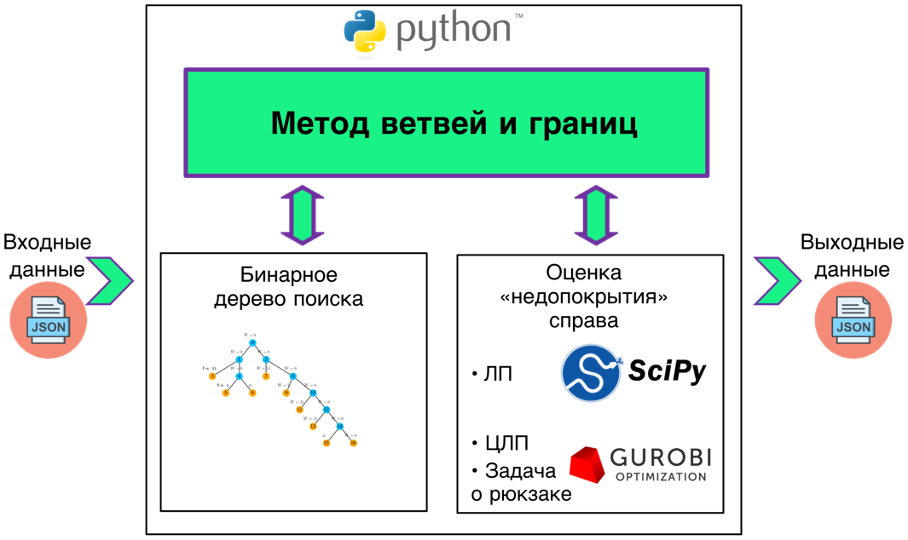
\includegraphics[width=.95\textwidth]{program_computer.png}
  \caption{Cтруктура программно-вычислительного комплекса}
  \label{fig:synopsis_program_computer}
  \end{figure}

Результаты численного сравнения решения задачи размещения БС с помощью предложенного алгоритма  типа ветвей и границ представлены в таблице \cref{tab:synopsis_models_comparation}. Рассматривался частный случай задачи, когда необходимо разместить весь набор заданных БС. Это необходимо, для того чтобы оценивать эффективность только предложенного алгоритма без учета влияния решения \textbf{задачи 2}. Поэтому оценка недопокрытия справа рассчитывается как

\begin{displaymath}
w_2 \left(G_\nu \right) = max\{\left(l_{n+1}-l_k\right)-(r_t+\sum_{j\in S_v}{2 \cdot r_j}),0\},
\end{displaymath}
где $S_\beta$ подмножества еще неразмещенных станций, $r_t$ -- радиус покрытия размещаемой БС $S_t$, $l_k$ -- координата точки размещения $a_k$. Чтобы сравнить результаты решения с помощью разработанного алгоритма с результатом решение задачи в виде ЦЛП, ограничение на время задержки не учитывалась.

Общее количество $\gamma$ вариантов расстановки $m$ станций по $n$ точкам размещения равна 

\begin{equation}
  \label{eq:synopsis_gamma}
  \gamma = C^m_n \cdot m! .
\end{equation}

  
Задача решалась с помощью метода ветвей и границ (МВиГ) для сформулированной комбинаторной модели, в виде сформулированной задачи ЦЛП, а также методом полного перебора (МПП). Для каждого набора мест размещения $n$ и множества БС $m$  было рассчитано по 10 примеров с различными параметрами БС. В таблице приводятся усредненные показатели числа просмотренных вершин дерева. В первом эксперименте для числа точек размещения $n=7$ и числа БС $m=4$ общее число вариантов расстановок по формуле \cref{eq:synopsis_gamma} $\gamma = 840$. Было рассчитано 10 примеров задачи с различными параметрами БС для каждого метода. Среднее число пройденных вершин $\nu$ при решении МПП составило 3122, МВиГ составило 360. Для задачи ЦЛП  среднее число пройденных узлов составило 275, что меньше чем в решении, полученном с помощью МВиГ. При увеличении размерности задачи, при $n=11$ и $m=6$,  для МВиГ число пройденных узлов составило $\nu = 88002$, что меньше практически в пять раз, чем при решении с помощью задачи ЦЛП $\nu=413767$.

Как видно из результатов сравнения, при увеличении размерности задачи предложенный в диссертационной работе алгоритм типа ветвей и границ показывает лучшие результаты по сравнению с результатом решения математической модели с помощью стандартных алгоритмов решения задачи ЦЛП в каноническом виде в программных пакетах.



\begin{table}
\caption{Результаты численного сравнения.}\label{tab:synopsis_models_comparation}
\begin{tabular}{|c|c|c|*{3}{l}|} \cline{3-6}
\hline
    \textbf{Число} & \textbf{Число} &\textbf{Число вариантов} & \multicolumn{3}{c|}{\textbf{Число пройденных}}\\ 

\textbf{точек, $n$} & \textbf{БС, $m$} &\textbf{расстановок, $\gamma$} & \multicolumn{3}{c|}{\textbf{узлов,} $\mathbf{\nu}$}\\ 
% \textbf{размещения,} & \textbf{cтанций,} & \textbf{вариантов} & \multicolumn{3}{c|}{\textbf{узлов дерева поиска, $\nu$}}\\
\cline{4-6}
    &  & & \textbf{МПП}& \textbf{МВиГ} & \textbf{ЦЛП} \\ 
\hline
7 &     4 & 840     & 3122 & 360 &  \textbf{275} \\
7 &     5 & 2 520   & 16114 & 560  &  \textbf{45}  \\
7 &     6 & 5 040   & 59564 & 364  &  \textbf{19}  \\
8 &     4 & 1 680   & 4954 &  434 &   \textbf{189} \\
8 &     5 & 6 720   & 6720 & \textbf{852}  &  878 \\
8 &     6 & 20 160  & 159170 & 592  & \textbf{185}  \\
9  &    4 & 3 024   & 9882 & \textbf{458} & 5511 \\
9  &    5 & 15 120  & 58190 &  \textbf{768} &  1236\\
9  &    6 & 60 480  & 366512 &  \textbf{720} & 13294 \\
10 &    4 & 5 040   & 14868&  \textbf{800}&  6243\\
10 &    5 & 30 240  & 113932&  \textbf{414}&  8043\\
10 &	6 & 151 200 & 828952&  \textbf{40872}&  71587\\
11 &    4 & 7 920   & 23482&  \textbf{354} & 15538\\
11 &	5 & 55 440  & 204894& \textbf{9138}&  74440\\
11 &	6 & 332 640 & 1592500 & \textbf{88002} & 413767 \\
\hline
\end{tabular}
\end{table} 
\normalsize



\FloatBarrier
\pdfbookmark{Заключение}{conclusion}                                  % Закладка pdf
В \underline{\textbf{заключении}} приведены основные результаты работы:
%% Согласно ГОСТ Р 7.0.11-2011:
%% 5.3.3 В заключении диссертации излагают итоги выполненного исследования, рекомендации, перспективы дальнейшей разработки темы.
%% 9.2.3 В заключении автореферата диссертации излагают итоги данного исследования, рекомендации и перспективы дальнейшей разработки темы.

\begin{enumerate}
    \item Проведен анализ методики проектирования современных БШС. В рамках такой методики были исследованы проблемы синтеза топологии БШС вдоль протяженных транспортных магистралей: автомобильные дороги, трубопроводные магистрали, лини метрополитена и т.д. 
    \item Предложена новая математическая модель в виде задачи ЦЛП оптимального размещения БС с линейной топологией.
    \item Представлена новая математическая модель задачи оптимального размещения БС в комбинаторной форме. 
    % Данная модель учитывает специфику задачи для нахождения оптимального решения.
    \item Для комбинаторной модели был разработан новый специальный алгоритм типа ветвей и границ. 
    
    % Представлены результаты сравнения поиска оптимального решения с помощью МВиГ с алгоритмами решения задачи в общем виде.
    \item В рамках комплексного проектирования БШС представлена новая итерационная процедура нахождения последовательности лучших решений задачи оптимального размещения БС для случая, когда найденное оптимальное решение построение топологии сети не удовлетворяет некоторым критериями функционирования БШС, проверяемых на следующих этапах проектирования.
    \item Предложена новая математическая модель виде задачи ЧЦЛП оптимального размещения БС для покрытия множества рассредоточенных объектов. 
    \item Разработан программный комплекс для расчета задачи оптимального размещения БС  с помощью предложенного алгоритма типа ветвей и границ.
    \item Представлены результаты численных экспериментов, доказывающие эффективность предложенных моделей и методов для решения задачи синтеза топологии при проектировании БШС.
\end{enumerate}

% \begin{enumerate}
%     \item Был проведен анализ методики проектирования современных БШС. В рамках такой методики были исследованы проблемы синтеза топологии БШС вдоль протяженных участков: трубопроводные магистрали, протяженные автомобильные дороги. 
%     \item Была предложена математическая модель в виде задачи ЦЛП размещения БС с линейной топологией.
%     \item Была представлена математическая модель экстремальной задачи оптимального размещения БС в комбинаторной форме. 
%     % Данная модель учитывает специфику задачи для нахождения оптимального решения.
%     \item Для комбинаторной модели был разработан специальный алгоритм типа ветвей и границ. Представлены результаты сравнения поиска оптимального решения с помощью МВиГ с алгоритмами решения задачи в общем виде.
%     \item В рамках комплексного проектирования была представлена итерационная процедура нахождения последовательности лучших решений задачи оптимального размещения для случая, когда найденное оптимальное решение построение топологии сети не удовлетворяет некоторым критериями функционирования БШС, проверяемых на этапе моделирования процесса передачи данных.
%     \item Предложена математическая модель оптимального размещения БС для покрытия множества рассредоточенных объектов.
%     \item Разработан программный комплекс для расчета задачи оптимального размещения БС  с помощью предложенного алгоритма типа ветвей и границ.
% \end{enumerate}




% \begin{enumerate}
%   \item построены математические модели в виде экстремальной комбинаторной задачи и задачи ЦЛП для оптимального размещения базовых станций при проектировании БШС с линейной топологией;
%   \item представлен алгоритм метода ветвей и границ для задачи размещения базовых станций с линейной топологией; 
%   \item разработана итерационная процедура нахождения последовательности лучших решений для задачи размещения базовых станций в рамках комплексного проектирования БШС с линейной топологией;
%   \item разработаны математические модели для задач проектирования БШС для покрытия множества рассредоточенныз объектов;
%   \item разработаны модели прогнозирования оценок характеристик производительности сети с помощью методов машинного обучения.
% \end{enumerate}


\pdfbookmark{Литература}{bibliography}                                % Закладка pdf
% При использовании пакета \verb!biblatex! список публикаций автора по теме
% диссертации формируется в разделе <<\publications>>\ файла
% \verb!common/characteristic.tex!  при помощи команды \verb!\nocite!

\ifdefmacro{\microtypesetup}{\microtypesetup{protrusion=false}}{} % не рекомендуется применять пакет микротипографики к автоматически генерируемому списку литературы
\urlstyle{rm}                               % ссылки URL обычным шрифтом
\ifnumequal{\value{bibliosel}}{0}{% Встроенная реализация с загрузкой файла через движок bibtex8
    \renewcommand{\bibname}{\large \bibtitleauthor}
    \nocite{*}
    \insertbiblioauthor           % Подключаем Bib-базы
    %\insertbiblioexternal   % !!! bibtex не умеет работать с несколькими библиографиями !!!
}{% Реализация пакетом biblatex через движок biber
    % Цитирования.
    %  * Порядок перечисления определяет порядок в библиографии (только внутри подраздела, если `\insertbiblioauthorgrouped`).
    %  * Если не соблюдать порядок "как для \printbibliography", нумерация в `\insertbiblioauthor` будет кривой.
    %  * Если цитировать каждый источник отдельной командой --- найти некоторые ошибки будет проще.
    %

    %% authorvak
    \nocite{IvanovVAK2019}%
    % TODO: доделать ссылку, после публикации
    \nocite{PershinVAK2022}
    %
    %% authorwos
    % \nocite{wosbib1}%
    %
    %% authorscopus
    % \nocite{scbib1}%
    \nocite{Ivanov2019}%
    \nocite{Larionov2021}

    
    \nocite{Mukhtarov2020}%
    %
    %% authorpathent
    % \nocite{patbib1}%
    %
    %% authorprogram
    \nocite{progbib_mukhtarpov}%
    %
    %% authorconf
    \nocite{MukhtarovSokolovITTMM2021}
    \nocite{VishnevskyMukhtarovPershinDCCN2020_RSCI}
    \nocite{LazarevaLarionovMukhtarovITTMM2020_RSCI}
    \nocite{MukhtarovIvanovPershinDCCN2019_RSCI}
    \nocite{MukhtarovPershinVSPU2019_RSCI}
    \nocite{MukhtarovPershinMLSD2019materials_RSCI}
    \nocite{MukhtarovPershinMLSD2019works_RSCI}
    %
    %% authorother
    \nocite{VishnevskyLarionovMukhtarovICAM2020_RSCI}
    \nocite{MukhtarovPershinGUBKIN2019_RSCI}
    \nocite{MukhtarovPershinGUBKIN2018_RSCI}%


    \ifnumgreater{\value{usefootcite}}{0}{
        \begin{refcontext}[labelprefix={}]
            \ifnum \value{bibgrouped}>0
                \insertbiblioauthorgrouped    % Вывод всех работ автора, сгруппированных по источникам
            \else
                \insertbiblioauthor      % Вывод всех работ автора
            \fi
        \end{refcontext}
    }{
        \ifnum \totvalue{citeexternal}>0
            % \begin{refcontext}[labelprefix=A]
            \begin{refcontext}
                \ifnum \value{bibgrouped}>0
                    \insertbiblioauthorgrouped    % Вывод всех работ автора, сгруппированных по источникам
                \else
                    \insertbiblioauthor      % Вывод всех работ автора
                \fi
            \end{refcontext}
        \else
            \ifnum \value{bibgrouped}>0
                \insertbiblioauthorgrouped    % Вывод всех работ автора, сгруппированных по источникам
            \else
                \insertbiblioauthor      % Вывод всех работ автора
            \fi
        \fi
        %  \insertbiblioauthorimportant  % Вывод наиболее значимых работ автора (определяется в файле characteristic во второй section)
        \begin{refcontext}[labelprefix={}]
            \insertbiblioexternal            % Вывод списка литературы, на которую ссылались в тексте автореферата
        \end{refcontext}
        % Невидимый библиографический список для подсчёта количества внешних публикаций
        % Используется, чтобы убрать приставку "А" у работ автора, если в автореферате нет
        % цитирований внешних источников.
        \printbibliography[heading=nobibheading, section=0, env=countexternal, keyword=biblioexternal, resetnumbers=true]%
    }
}
\ifdefmacro{\microtypesetup}{\microtypesetup{protrusion=true}}{}
\urlstyle{tt}                               % возвращаем установки шрифта ссылок URL